%--------------------------------------
%ELECTROTECHNIQUE - SCHEMA DE LIAISON A LA TERRE
%--------------------------------------

%--------------------------------------
%appel de la classe de document et de ses options
%--------------------------------------

\documentclass[a4paper, 11pt, twoside, fleqn, french]{memoir}

\usepackage{AOCDTF}

\addbibresource{../../../parametres/bibliographies/bib_electrotechnique.bib}

%--------------------------------------
%données du document
%--------------------------------------

\title{\'Electrotechnique -- Schéma de liaison à la terre}
\date{\year}
\author[1]{Bruno Douchy}
%\author[2]{Prénom2 Nom2}
%\author[3]{Prénom3 Nom3}
%\author[4]{Prénom4 Nom4}

%--------------------------------------
%programmations spécifiques de mise-en-pages adaptables selon les matières et bibliographie
%--------------------------------------

%--------------------------------------
%CANEVAS
%--------------------------------------

\newcommand\BoxColor{\ifcase\thechapshift blue!30\or brown!30\or pink!30\or cyan!30\or green!30\or teal!30\or purple!30\or red!30\or olive!30\or orange!30\or lime!30\or gray!\or magenta!30\else yellow!30\fi} %définition de la couleur des marqueurs de chapitre

\newcounter{chapshift} %compteur de chapitre du marqueur de chapitre
\addtocounter{chapshift}{-1}
	
\newif\ifFrame %instruction conditionnelle pour les couleurs des pages
\Frametrue

\pagestyle{plain}

% the main command; the mandatory argument sets the color of the vertical box
\newcommand\ChapFrame{%
\AddEverypageHook{%
\ifFrame
\ifthenelse{\isodd{\value{page}}}
  {\backgroundsetup{contents={%
  \begin{tikzpicture}[overlay,remember picture]
  \node[
  	rounded corners=3pt,
    fill=\BoxColor,
    inner sep=0pt,
    rectangle,
    text width=1.3cm,
    text height=5.5cm,
    align=center,
    anchor=north west
  ] 
  at ($ (current page.north west) + (-0cm,-2*\thechapshift cm) $) %nombre négatif = espacement des marqueurs entre les différents chapitres (à régler en fin de rédaction) (4.5cm vaut un espacement équivalement à la hauteur du marqueur, une page peut en contenir 6 avec cet espacement-la mais il est le plus équilibré)
    {\rotatebox{90}{\hspace*{.3cm}%
      \parbox[c][0.9cm][t]{5cm}{%
        \raggedright\textcolor{black}{\sffamily\textbf{\leftmark}}}}};
  \end{tikzpicture}}}
  }
  {\backgroundsetup{contents={%
  \begin{tikzpicture}[overlay,remember picture]
  \node[
  	rounded corners=3pt,
    fill=\BoxColor,
    inner sep=0pt,
    rectangle,
    text width=1.3cm,
    text height=5.5cm,
    align=center,
    anchor=north east
  ] 
  at ($ (current page.north east) + (-0cm,-2*\thechapshift cm) $) %nombre négatif = espacement des marqueurs entre les différents chapitres (à régler en fin de rédaction) (4.5cm vaut un espacement équivalement à la hauteur du marqueur, une page peut en contenir 6 avec cet espacement-la mais il est le plus équilibré)
    {\rotatebox{90}{\hspace*{.3cm}%
      \parbox[c][0.9cm][t]{5cm}{%
        \raggedright\textcolor{black}{\sffamily\textbf{\leftmark}}}}};
  \end{tikzpicture}}}%
  }
  \BgMaterial%
  \fi%
}%
  \stepcounter{chapshift}
}

\renewcommand\chaptermark[1]{\markboth{\thechapter.~#1}{}} %redéfinition du marqueur de chapitre pour ne contenir que le titre du chapitre %à personnaliser selon le nombre de chapitre dans le cours

%--------------------------------------
%corps du document
%--------------------------------------

\begin{document} %corps du document

%--------------------------------------
%préface, page de couverture, table des matières...
%--------------------------------------

\frontmatter
	
\openleft %début de chapitre à gauche
\Framefalse %défini la booléenne Frame comme faux
\Invnumtrue %défini la booléenne Invnum comme vrai -> inversion des numéros de pages
	
	%--------------------------------------
	%page de couverture et de titre
	%--------------------------------------

	%--------------------------------------
%CANEVAS
%--------------------------------------

%utiliser les environnement \begin{comment} \end{comment} pour mettre en commentaire le préambule une fois la programmation appelée dans le document maître (!ne pas oublier de mettre en commentaire \end{document}!)

\begin{comment}

\documentclass[a4paper, 11pt, twoside, fleqn]{memoir}

\usepackage{AOCDTF}

%--------------------------------------
%CANEVAS
%--------------------------------------

\newcommand\BoxColor{\ifcase\thechapshift blue!30\or brown!30\or pink!30\or cyan!30\or green!30\or teal!30\or purple!30\or red!30\or olive!30\or orange!30\or lime!30\or gray!\or magenta!30\else yellow!30\fi} %définition de la couleur des marqueurs de chapitre

\newcounter{chapshift} %compteur de chapitre du marqueur de chapitre
\addtocounter{chapshift}{-1}
	
\newif\ifFrame %instruction conditionnelle pour les couleurs des pages
\Frametrue

\pagestyle{plain}

% the main command; the mandatory argument sets the color of the vertical box
\newcommand\ChapFrame{%
\AddEverypageHook{%
\ifFrame
\ifthenelse{\isodd{\value{page}}}
  {\backgroundsetup{contents={%
  \begin{tikzpicture}[overlay,remember picture]
  \node[
  	rounded corners=3pt,
    fill=\BoxColor,
    inner sep=0pt,
    rectangle,
    text width=1.3cm,
    text height=5.5cm,
    align=center,
    anchor=north west
  ] 
  at ($ (current page.north west) + (-0cm,-2*\thechapshift cm) $) %nombre négatif = espacement des marqueurs entre les différents chapitres (à régler en fin de rédaction) (4.5cm vaut un espacement équivalement à la hauteur du marqueur, une page peut en contenir 6 avec cet espacement-la mais il est le plus équilibré)
    {\rotatebox{90}{\hspace*{.3cm}%
      \parbox[c][0.9cm][t]{5cm}{%
        \raggedright\textcolor{black}{\sffamily\textbf{\leftmark}}}}};
  \end{tikzpicture}}}
  }
  {\backgroundsetup{contents={%
  \begin{tikzpicture}[overlay,remember picture]
  \node[
  	rounded corners=3pt,
    fill=\BoxColor,
    inner sep=0pt,
    rectangle,
    text width=1.3cm,
    text height=5.5cm,
    align=center,
    anchor=north east
  ] 
  at ($ (current page.north east) + (-0cm,-2*\thechapshift cm) $) %nombre négatif = espacement des marqueurs entre les différents chapitres (à régler en fin de rédaction) (4.5cm vaut un espacement équivalement à la hauteur du marqueur, une page peut en contenir 6 avec cet espacement-la mais il est le plus équilibré)
    {\rotatebox{90}{\hspace*{.3cm}%
      \parbox[c][0.9cm][t]{5cm}{%
        \raggedright\textcolor{black}{\sffamily\textbf{\leftmark}}}}};
  \end{tikzpicture}}}%
  }
  \BgMaterial%
  \fi%
}%
  \stepcounter{chapshift}
}

\renewcommand\chaptermark[1]{\markboth{\thechapter.~#1}{}} %redéfinition du marqueur de chapitre pour ne contenir que le titre du chapitre %à personnaliser selon le nombre de chapitre dans le cours

%--------------------------------------
%corps du document
%--------------------------------------

\begin{document} %corps du document
	\openleft %début de chapitre à gauche

\end{comment}

\pagestyle{empty}

\begingroup

%--------------------------------------
%arrière-plan
%--------------------------------------
	\begin{tikzpicture}[remember picture, overlay]
		\begin{scope}[shift={(current page.south west)}]
			\draw[draw=lightgray,fill=lightgray] (0,0) rectangle (21,30);
		\end{scope}
	\end{tikzpicture}

%--------------------------------------
%bandeau vertical
%--------------------------------------

	\begin{tikzpicture}[remember picture, overlay]
		\begin{scope}[shift={(current page.south west)}]
			\draw[draw=orangelogo,fill=orangelogo, opacity=0.7] (0,0) rectangle (4,30);
		\end{scope}
	\end{tikzpicture}

%--------------------------------------
%texte dans bandeau vertical
%--------------------------------------
  
	\begin{tikzpicture}[remember picture, overlay]
	\begin{scope}[shift={(current page.south west)}]
			\draw (1.8,1) node [right, rotate=90, opacity=0.7] {\sffamily\textbf{\Large\color{bleulogo}M\'ETIERS DES TECHNOLOGIES ASSOCI\'EES}};
			\draw (2.5,1) node [right, rotate=90, opacity=0.7] {\sffamily\textbf{\Large\color{bleulogo}ASSOCIATION OUVRIÈRE DES COMPAGNONS DU DEVOIR ET DU TOUR DE FRANCE}};
			\draw (3.4,29) node [left, rotate=90, opacity=0.7] {\sffamily\textls[200]{\Huge\textbf{\color{bleulogo}BTS \'ELECTROTECHNIQUE}}};
		\end{scope}
	\end{tikzpicture}

%--------------------------------------
%titre 
%--------------------------------------

	\begin{tikzpicture}[remember picture, overlay]
		\begin{scope}[shift={(current page.north west)}]
		%\draw (5,-12.5) node [right] {\sffamily\textls[150]{\Huge\textbf{\color{darkgray}\textsc{Matière ligne1}}}}; 	%ligne 1 long intitulé de la matière
		\draw (5,-14) node [right, opacity=0.7] {\sffamily\textls[150]{\Huge\textbf{\color{bleulogo}\'Electrotechnique}}}; %intitulé de la matière
		\draw (20,-16) node [left, opacity=0.7] {\sffamily\textls[150]{\Huge\textbf{\color{bleulogo}Schéma de liaison}}}; %intitulé du cours
		\draw (20,-17.5) node [left, opacity=0.7] {\sffamily\textls[150]{\Huge\textbf{\color{bleulogo}\textsc{à la terre}}}};  %ligne 1 long intitulé du cours
		\draw[very thick, orangelogo, opacity=0.7] (5,-15) -- (20,-15);
		\end{scope}
	\end{tikzpicture}

%--------------------------------------
%logo
%--------------------------------------

	\begin{tikzpicture}[remember picture, overlay]
		\begin{scope}[shift={(current page.north west)}]
			\draw (12.5,-7) %(12.5, -6) si long intitulé du chapitre
			node [opacity=0.3] {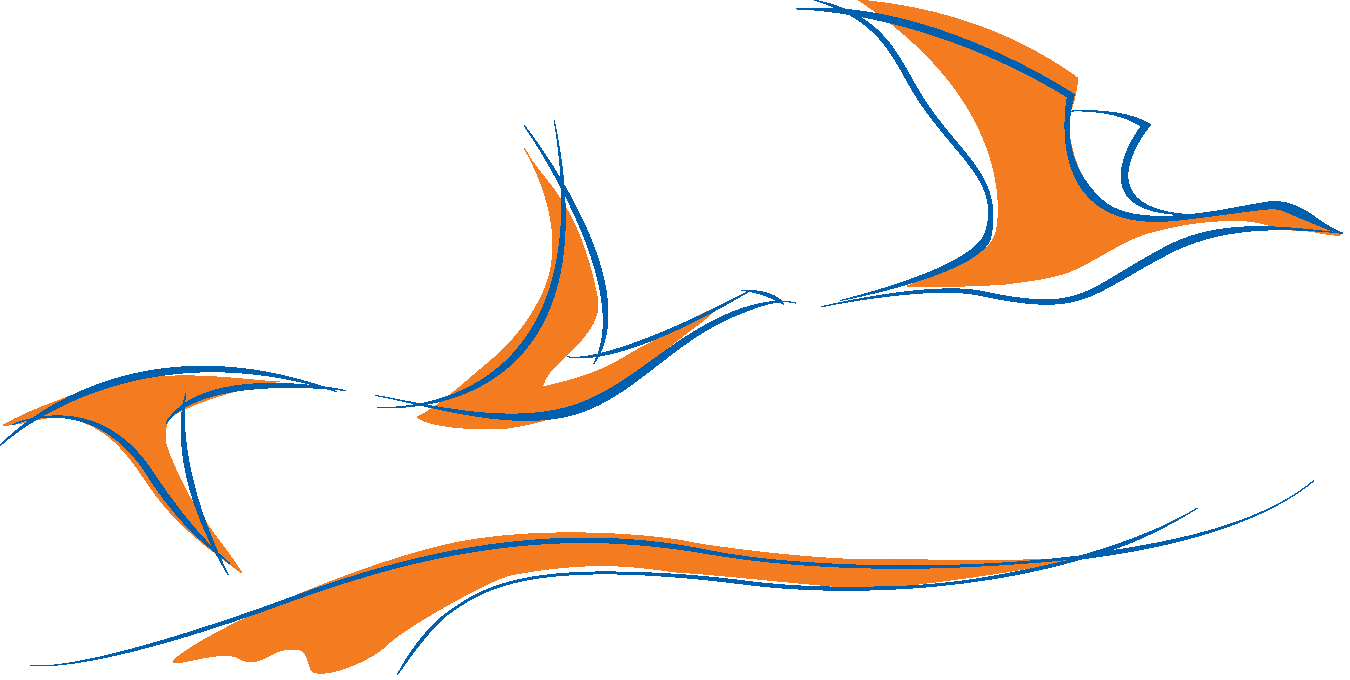
\includegraphics[scale=0.3]{logo_compagnons}};
			\draw (12.5,-23) %(12.5, -24) si long intitulé du chapitre
			node [opacity=0.3] {
\includegraphics[scale=0.7]{logo_metier}};
		\end{scope}
	\end{tikzpicture}

\endgroup

\null\cleardoublepage

%\end{document}

	%--------------------------------------
%CANEVAS
%--------------------------------------

%utiliser les environnement \begin{comment} \end{comment} pour mettre en commentaire le préambule une fois la programmation appelée dans le document maître (!ne pas oublier de mettre en commentaire \end{document}!)

\begin{comment}

\documentclass[a4paper, 11pt, twoside, fleqn]{memoir}

\usepackage{AOCDTF}

%--------------------------------------
%CANEVAS
%--------------------------------------

\newcommand\BoxColor{\ifcase\thechapshift blue!30\or brown!30\or pink!30\or cyan!30\or green!30\or teal!30\or purple!30\or red!30\or olive!30\or orange!30\or lime!30\or gray!\or magenta!30\else yellow!30\fi} %définition de la couleur des marqueurs de chapitre

\newcounter{chapshift} %compteur de chapitre du marqueur de chapitre
\addtocounter{chapshift}{-1}
	
\newif\ifFrame %instruction conditionnelle pour les couleurs des pages
\Frametrue

\pagestyle{plain}

% the main command; the mandatory argument sets the color of the vertical box
\newcommand\ChapFrame{%
\AddEverypageHook{%
\ifFrame
\ifthenelse{\isodd{\value{page}}}
  {\backgroundsetup{contents={%
  \begin{tikzpicture}[overlay,remember picture]
  \node[
  	rounded corners=3pt,
    fill=\BoxColor,
    inner sep=0pt,
    rectangle,
    text width=1.3cm,
    text height=5.5cm,
    align=center,
    anchor=north west
  ] 
  at ($ (current page.north west) + (-0cm,-2*\thechapshift cm) $) %nombre négatif = espacement des marqueurs entre les différents chapitres (à régler en fin de rédaction) (4.5cm vaut un espacement équivalement à la hauteur du marqueur, une page peut en contenir 6 avec cet espacement-la mais il est le plus équilibré)
    {\rotatebox{90}{\hspace*{.3cm}%
      \parbox[c][0.9cm][t]{5cm}{%
        \raggedright\textcolor{black}{\sffamily\textbf{\leftmark}}}}};
  \end{tikzpicture}}}
  }
  {\backgroundsetup{contents={%
  \begin{tikzpicture}[overlay,remember picture]
  \node[
  	rounded corners=3pt,
    fill=\BoxColor,
    inner sep=0pt,
    rectangle,
    text width=1.3cm,
    text height=5.5cm,
    align=center,
    anchor=north east
  ] 
  at ($ (current page.north east) + (-0cm,-2*\thechapshift cm) $) %nombre négatif = espacement des marqueurs entre les différents chapitres (à régler en fin de rédaction) (4.5cm vaut un espacement équivalement à la hauteur du marqueur, une page peut en contenir 6 avec cet espacement-la mais il est le plus équilibré)
    {\rotatebox{90}{\hspace*{.3cm}%
      \parbox[c][0.9cm][t]{5cm}{%
        \raggedright\textcolor{black}{\sffamily\textbf{\leftmark}}}}};
  \end{tikzpicture}}}%
  }
  \BgMaterial%
  \fi%
}%
  \stepcounter{chapshift}
}

\renewcommand\chaptermark[1]{\markboth{\thechapter.~#1}{}} %redéfinition du marqueur de chapitre pour ne contenir que le titre du chapitre %à personnaliser selon le nombre de chapitre dans le cours

%--------------------------------------
%corps du document
%--------------------------------------

\begin{document} %corps du document
	\openleft %début de chapitre à gauche

\end{comment}

\pagestyle{empty}
\thispagestyle{empty}

\begingroup

%--------------------------------------
%logo Compagnon
%--------------------------------------
 
\begin{tikzpicture}[remember picture, overlay]
	\begin{scope}[shift={(current page.north west)}]
		\draw (1,-1)
		node [below right]{
\includegraphics[scale=0.1]{logo_compagnons_nom.png}};
	\end{scope}
\end{tikzpicture}

~\\[5cm] %espace insécable pour marquer le début du texte sur l'environnement et situer d'autres éléments de texte sur la page

%--------------------------------------
%titre de la page
%--------------------------------------

\begin{flushleft}
	\HUGE\sffamily\textbf{Matière}\\
\end{flushleft}
\HRule
\begin{flushright}
	\huge\sffamily\textbf{Cours}\\[0.4cm]
\end{flushright}
~\\[2cm]

%--------------------------------------
%auteur et logo MTA
%--------------------------------------

\begin{minipage}{0.3\textwidth}
 \noindent\large
		\rmfamily Prénom1 \textsc{Nom1}
		\\
		\rmfamily Prénom2 \textsc{Nom2}
\end{minipage}
\hfill
\begin{minipage}{0.3\textwidth}
	\centering
	
\includegraphics[scale=0.25]{logo_metier.png}
\end{minipage}

\begin{comment}
\hfill
\begin{minipage}{0.3\textwidth}
	\begin{flushright} \large
		\rmfamily Prénom3 \textsc{Nom3} %auteur supplémentaires à rajouter en mettant en commentaire l'environnement comment
		\\
 		\rmfamily Prénom4 \textsc{Nom4}
	\end{flushright}
\end{minipage}
\end{comment}

\vfill
\begin{flushleft}
	\sffamily\bfseries\large\ Édition \the\year.\the\month
\end{flushleft}
\vfill

%--------------------------------------
%pied de page Compagnon
%--------------------------------------

\begin{tikzpicture}[remember picture, overlay]
	\begin{scope}[shift={(current page.south west)}]
		\draw (1,0)
		node [above right]{
\includegraphics{pied_page_compagnons.png}};
	\end{scope}
\end{tikzpicture}

\endgroup
\null\clearpage

%\end{document}

	\pagestyle{plain} %style de page avec en-tête et pied-de-page
	\pagenumbering{roman}

	%--------------------------------------
	%listes de contenus
	%--------------------------------------
	
	{\hypersetup{linkcolor=black}\tableofcontents} %table des matières en noir
	\newpage
	{\hypersetup{linkcolor=black}\listoftables} %liste des figures en noir
	\newpage
	{\hypersetup{linkcolor=black}\listoffigures} %liste des tableaux en noir
	{\hypersetup{linkcolor=black}\listofequations} %liste des équations en noir

	%--------------------------------------
	%chapitre d'introduction
	%--------------------------------------
	
%--------------------------------------
%corps de texte, annexes
%--------------------------------------

\let\clearpage %supprime une page blanche en cas double page avant le corps du texte
 
\mainmatter

\Frametrue %défini la booléenne Frame comme vrai -> marqueurs de chapitre
\Invnumfalse %défini la booléenne Invnum comme faux

	%--------------------------------------
	%inclusion des chapitres
	%--------------------------------------

	%--------------------------------------
%ELECTROTECHNIQUE - SCHEMA DE LIAISON A LA TERRE
%--------------------------------------

%utiliser les environnement \begin{comment} \end{comment} pour mettre en commentaire le préambule une fois la programmation appelée dans le document maître (!ne pas oublier de mettre en commentaire \end{document}!)

\begin{comment}

\documentclass[a4paper, 11pt, twoside, fleqn]{memoir}

\usepackage{AOCDTF}

%--------------------------------------
%CANEVAS
%--------------------------------------

\newcommand\BoxColor{\ifcase\thechapshift blue!30\or brown!30\or pink!30\or cyan!30\or green!30\or teal!30\or purple!30\or red!30\or olive!30\or orange!30\or lime!30\or gray!\or magenta!30\else yellow!30\fi} %définition de la couleur des marqueurs de chapitre

\newcounter{chapshift} %compteur de chapitre du marqueur de chapitre
\addtocounter{chapshift}{-1}
	
\newif\ifFrame %instruction conditionnelle pour les couleurs des pages
\Frametrue

\pagestyle{plain}

% the main command; the mandatory argument sets the color of the vertical box
\newcommand\ChapFrame{%
\AddEverypageHook{%
\ifFrame
\ifthenelse{\isodd{\value{page}}}
  {\backgroundsetup{contents={%
  \begin{tikzpicture}[overlay,remember picture]
  \node[
  	rounded corners=3pt,
    fill=\BoxColor,
    inner sep=0pt,
    rectangle,
    text width=1.3cm,
    text height=5.5cm,
    align=center,
    anchor=north west
  ] 
  at ($ (current page.north west) + (-0cm,-2*\thechapshift cm) $) %nombre négatif = espacement des marqueurs entre les différents chapitres (à régler en fin de rédaction) (4.5cm vaut un espacement équivalement à la hauteur du marqueur, une page peut en contenir 6 avec cet espacement-la mais il est le plus équilibré)
    {\rotatebox{90}{\hspace*{.3cm}%
      \parbox[c][0.9cm][t]{5cm}{%
        \raggedright\textcolor{black}{\sffamily\textbf{\leftmark}}}}};
  \end{tikzpicture}}}
  }
  {\backgroundsetup{contents={%
  \begin{tikzpicture}[overlay,remember picture]
  \node[
  	rounded corners=3pt,
    fill=\BoxColor,
    inner sep=0pt,
    rectangle,
    text width=1.3cm,
    text height=5.5cm,
    align=center,
    anchor=north east
  ] 
  at ($ (current page.north east) + (-0cm,-2*\thechapshift cm) $) %nombre négatif = espacement des marqueurs entre les différents chapitres (à régler en fin de rédaction) (4.5cm vaut un espacement équivalement à la hauteur du marqueur, une page peut en contenir 6 avec cet espacement-la mais il est le plus équilibré)
    {\rotatebox{90}{\hspace*{.3cm}%
      \parbox[c][0.9cm][t]{5cm}{%
        \raggedright\textcolor{black}{\sffamily\textbf{\leftmark}}}}};
  \end{tikzpicture}}}%
  }
  \BgMaterial%
  \fi%
}%
  \stepcounter{chapshift}
}

\renewcommand\chaptermark[1]{\markboth{\thechapter.~#1}{}} %redéfinition du marqueur de chapitre pour ne contenir que le titre du chapitre %à personnaliser selon le nombre de chapitre dans le cours

%--------------------------------------
%corps du document
%--------------------------------------

\begin{document} %corps du document
	\openleft %début de chapitre à gauche

\end{comment}

\chapter{Les dangers de l'électricité}
\label{chap:dangers_electricite}
\ChapFrame %appel du marqueur de chapitre

\section{Catégories de tension}

\begin{table}[h]
\caption{Domaines de tensions\label{tab:categories_tension}}
\begin{threeparttable} %note dans tableau
\begin{tabularx}{\textwidth}{l C k@{${\enspace{}}U_n{\enspace{}}$}i k@{${\enspace{}}U_n{\enspace{}}$}i} %les deux derniers,types de colonne sont deux colonnes compactées avec la lettre U comme colonne du centre
\toprule
\multicolumn{2}{c}{\thead{Domaine de tension}}	& \multicolumn{2}{c}{\thead[c]{Courant alternatif\tnote{\ 1}}}		&  \multicolumn{2}{c}{\thead[c]{Courant continu}} \\
\midrule
Très Basse Tension										& TBT		&						& \leq 50\volt				& 						& \leq 120\volt \\
Basse Tension												& BT			& 50\volt < 		& \leq 1000\volt			& 120\volt < 		& \leq 1500\volt \\
\multirow[t]{2}{*}{Haute Tension\tnote{2}}	& HTA		& 1000\volt < 	& \leq 50\kilo\volt		& 1500\volt < 	& \leq 75\kilo\volt \\
																	& HTB		&  					& > 50\kilo\volt			& 						& > 75\kilo\volt \\
\bottomrule
\end{tabularx}
\begin{tablenotes}
    \item[1] Tension nominale exprimée en \emph{valeur efficace} $U_n$\,;
    \item[2] Les basses tensions ne sont plus divisées en deux catégories depuis 2010, seule la haute tension conserve cette caractéristique.
\end{tablenotes}
\end{threeparttable}
\end{table}
	
\section{Action du courant électrique sur le corps humain}

Les dégâts provoqués au corps humain par un choc électrique sont directement corrélés à l'énergie dissipée par ce choc. Cette énergie dissipée est définie par la \emph{loi de Joule}.

\begin{equa} %environnement pour créer des équations référencées avec légendes alignée sur &=
	\begin{align} 
		W &= R \cdot I^{2} \cdot t
	\end{align}
\caption{Loi de Joule\label{eq:loi_joule}}
\end{equa}

\begin{textvariables}
R						& résistance										& hhm 						& \ohm								&\\
I						& courant électrique							& milliampère			& \milli\ampere					& \\
t						& durée												& seconde					& \second							&	\\
\end{textvariables}

La présence d'une tension électrique entraine toujours un risque de choc électrique mais il est peu aisé de déterminer un seuil de tension pour lequel le choc est dangereux car ce sont l'\emph{intensité} du courant $I$ traversant le corps et la \emph{durée} $t$ du choc électrique qui permettent de déterminer la probabilité de décès.\\

\begin{equa} %environnement pour créer des équations référencées avec légendes alignée sur &=
	\begin{align} 
		I &= \frac{116}{\sqrt{t}}
	\end{align}
\caption{Valeur statistique du courant entrainant la mort en fonction de la durée}
\label{eq:valeur_courant_mort}
\end{equa}

\begin{textvariables}
I						& courant électrique							& milliampère			& \milli\ampere					& 	Courant traversant le corps 	\\
t						& durée												& seconde					& \second							& 	Durée du choc électrique d'une durée ($8\milli\second < t \leq 5\second \nonumber$) \\
116					& constante										& / 							& 	/									& 	Constante empirique déterminée statistiquement\supercite{WildiSybille2014}\\
\end{textvariables}

En plus de l'intensité du courant et de la durée de passage du courant dans le corps, la surface de contact et la susceptibilité spécifique à chaque personne sont d'autres facteurs de gravité d'un contact électrique. Plus de précisions sur la prévention du danger électrique en \superref{sec:etat_lieux_prevention_electrique}.

\subsection{Effet du courant alternatif}

Les effets du courant alternatif entre \SI{15}{\hertz} et \SI{100}{\hertz} sont décrit en \autoref{fig:effets_courant_electrique_alternatif}. 

%--------------------------------------
%ELECTROTECHNIQUE - SCHEMA DE LIAISON A LA TERRE
%--------------------------------------

%utiliser les environnement \begin{comment} \end{comment} pour mettre en commentaire le préambule une fois la programmation appelée dans le document maître (!ne pas oublier de mettre en commentaire \end{document}!)

\begin{comment}

\documentclass[a4paper, 11pt, twoside, fleqn]{memoir}

\usepackage{AOCDTF}

%--------------------------------------
%CANEVAS
%--------------------------------------

\newcommand\BoxColor{\ifcase\thechapshift blue!30\or brown!30\or pink!30\or cyan!30\or green!30\or teal!30\or purple!30\or red!30\or olive!30\or orange!30\or lime!30\or gray!\or magenta!30\else yellow!30\fi} %définition de la couleur des marqueurs de chapitre

\newcounter{chapshift} %compteur de chapitre du marqueur de chapitre
\addtocounter{chapshift}{-1}
	
\newif\ifFrame %instruction conditionnelle pour les couleurs des pages
\Frametrue

\pagestyle{plain}

% the main command; the mandatory argument sets the color of the vertical box
\newcommand\ChapFrame{%
\AddEverypageHook{%
\ifFrame
\ifthenelse{\isodd{\value{page}}}
  {\backgroundsetup{contents={%
  \begin{tikzpicture}[overlay,remember picture]
  \node[
  	rounded corners=3pt,
    fill=\BoxColor,
    inner sep=0pt,
    rectangle,
    text width=1.3cm,
    text height=5.5cm,
    align=center,
    anchor=north west
  ] 
  at ($ (current page.north west) + (-0cm,-2*\thechapshift cm) $) %nombre négatif = espacement des marqueurs entre les différents chapitres (à régler en fin de rédaction) (4.5cm vaut un espacement équivalement à la hauteur du marqueur, une page peut en contenir 6 avec cet espacement-la mais il est le plus équilibré)
    {\rotatebox{90}{\hspace*{.3cm}%
      \parbox[c][0.9cm][t]{5cm}{%
        \raggedright\textcolor{black}{\sffamily\textbf{\leftmark}}}}};
  \end{tikzpicture}}}
  }
  {\backgroundsetup{contents={%
  \begin{tikzpicture}[overlay,remember picture]
  \node[
  	rounded corners=3pt,
    fill=\BoxColor,
    inner sep=0pt,
    rectangle,
    text width=1.3cm,
    text height=5.5cm,
    align=center,
    anchor=north east
  ] 
  at ($ (current page.north east) + (-0cm,-2*\thechapshift cm) $) %nombre négatif = espacement des marqueurs entre les différents chapitres (à régler en fin de rédaction) (4.5cm vaut un espacement équivalement à la hauteur du marqueur, une page peut en contenir 6 avec cet espacement-la mais il est le plus équilibré)
    {\rotatebox{90}{\hspace*{.3cm}%
      \parbox[c][0.9cm][t]{5cm}{%
        \raggedright\textcolor{black}{\sffamily\textbf{\leftmark}}}}};
  \end{tikzpicture}}}%
  }
  \BgMaterial%
  \fi%
}%
  \stepcounter{chapshift}
}

\renewcommand\chaptermark[1]{\markboth{\thechapter.~#1}{}} %redéfinition du marqueur de chapitre pour ne contenir que le titre du chapitre %à personnaliser selon le nombre de chapitre dans le cours

%--------------------------------------
%corps du document
%--------------------------------------

\begin{document} %corps du document
	\openleft %début de chapitre à gauche

\end{comment}

\begin{figure}
\centering
\caption{Effets du courant alternatif sur le corps humain \label{fig:effets_courant_electrique_alternatif}}
\begin{tikzpicture}
%\DrawGrid{(-7,-5)}{(7,5)} %grille d'aide pour le placement des objets

\draw (-7,4) node [right, minimum width=2cm, text width=1.8cm] {\footnotesize{Intensité de contact $I_c$}};
\draw [->] (-5,2.2) -- (-5,4);
\draw (-5, 2) node {\vdots};
\draw (-5,-3.9) -- (-5,1.6);

\draw (-5.4,-3) node [left] {\SI{0,5}{\milli\ampere}};
\draw [->] (-5.2,-3) -- (-4.5,-3);
\draw (-4.2,-3) node [anchor=mid west, text width=7cm] (A) {Sensation de picotements, de très faible à faible};
\draw (7,-3.5) node [anchor=east] {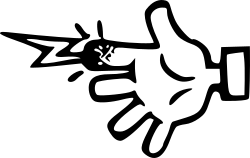
\includegraphics[width=2cm]{sensation}};

\draw (-5.4,-2.6) node [left] {\SI{10}{\milli\ampere}};
\draw [->] (-5.2,-2.6) -- (-4.5,-2.6);
\draw (-4.2,-2.6) node [anchor=mid west, text width=7cm] {Seuil de non lâcher, paralysie musculaire};
\draw (3.2,-2.6) node [anchor=west] {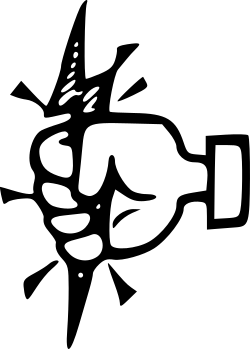
\includegraphics[width=1.5cm]{tetanisation}};

\draw (-5.4,-1.8) node [left] {\SI{30}{\milli\ampere}};
\draw [->] (-5.2,-1.8) -- (-4.5,-1.8);
\draw (-4.2,-1.8) node [anchor=mid west, text width=7cm] {Seuil de paralysie respiratoire};
\draw (7,-1.8) node [anchor=east] {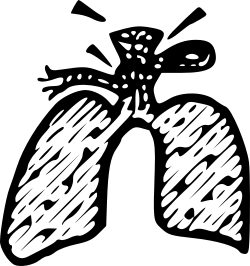
\includegraphics[width=1.5cm]{paralysie_poumon}};

\draw (-5.4,0.7) node [left] {\SI{75}{\milli\ampere}};
\draw [->] (-5.2,0.7) -- (-4.5,0.7);
\draw (-4.2,0.7) node [anchor=mid west, text width=7cm] {Seuil de fibriliation ventriculaire};
\draw (5.1,0.7) node {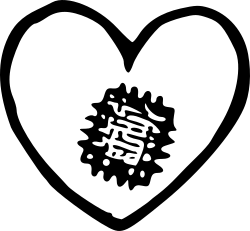
\includegraphics[width=1.5cm]{fibrillation}};

\draw (-5.4,3.1) node [left] {\SI{1}{\ampere}};
\draw [->] (-5.2,3.1) -- (-4.5,3.1);
\draw (-4.2,3.1) node [anchor=mid west, text width=7cm] {Arrêt du coeur};
\draw (5.2,3.1) node {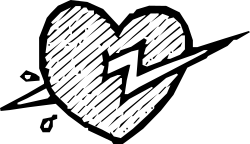
\includegraphics[width=2.4cm]{arret_cardiaque}};

\end{tikzpicture}
\end{figure}

%\end{document}

\subsubsection{Cas particuliers}

Pour le courant alternatifs d'une fréquence supérieures à \SI{100}{\hertz} :

\begin{itemize}
\item Plus la fréquence du courant augmente, plus les risques de fibrillation ventriculaire diminue\,;
\item Plus la fréquence du courant augmente, plus les risques de brûlures augmentent\,;
\item Plus la fréquence du courant augmente, plus l'impédance du corps humain diminue\,;
\item Il est généralement considéré que les conditions de protection contre les contacts indirects sont identiques que ça soit sous une fréquence de \SI{50}{\hertz} (réseau électrique domestique en Europe) où \SI{400}{\hertz} (réseau électrique des bateaux, avions, batmobile\ldots).
\end{itemize}

\subsection{Effet du courant continu}

Les effets du courant continus sont décrits en \autoref{fig:effets_courant_electrique_continu}.

%--------------------------------------
%ELECTROTECHNIQUE - SCHEMA DE LIAISON A LA TERRE
%--------------------------------------

%utiliser les environnement \begin{comment} \end{comment} pour mettre en commentaire le préambule une fois la programmation appelée dans le document maître (!ne pas oublier de mettre en commentaire \end{document}!)

\begin{comment}

\documentclass[a4paper, 11pt, twoside, fleqn]{memoir}

\usepackage{AOCDTF}

%--------------------------------------
%CANEVAS
%--------------------------------------

\newcommand\BoxColor{\ifcase\thechapshift blue!30\or brown!30\or pink!30\or cyan!30\or green!30\or teal!30\or purple!30\or red!30\or olive!30\or orange!30\or lime!30\or gray!\or magenta!30\else yellow!30\fi} %définition de la couleur des marqueurs de chapitre

\newcounter{chapshift} %compteur de chapitre du marqueur de chapitre
\addtocounter{chapshift}{-1}
	
\newif\ifFrame %instruction conditionnelle pour les couleurs des pages
\Frametrue

\pagestyle{plain}

% the main command; the mandatory argument sets the color of the vertical box
\newcommand\ChapFrame{%
\AddEverypageHook{%
\ifFrame
\ifthenelse{\isodd{\value{page}}}
  {\backgroundsetup{contents={%
  \begin{tikzpicture}[overlay,remember picture]
  \node[
  	rounded corners=3pt,
    fill=\BoxColor,
    inner sep=0pt,
    rectangle,
    text width=1.3cm,
    text height=5.5cm,
    align=center,
    anchor=north west
  ] 
  at ($ (current page.north west) + (-0cm,-2*\thechapshift cm) $) %nombre négatif = espacement des marqueurs entre les différents chapitres (à régler en fin de rédaction) (4.5cm vaut un espacement équivalement à la hauteur du marqueur, une page peut en contenir 6 avec cet espacement-la mais il est le plus équilibré)
    {\rotatebox{90}{\hspace*{.3cm}%
      \parbox[c][0.9cm][t]{5cm}{%
        \raggedright\textcolor{black}{\sffamily\textbf{\leftmark}}}}};
  \end{tikzpicture}}}
  }
  {\backgroundsetup{contents={%
  \begin{tikzpicture}[overlay,remember picture]
  \node[
  	rounded corners=3pt,
    fill=\BoxColor,
    inner sep=0pt,
    rectangle,
    text width=1.3cm,
    text height=5.5cm,
    align=center,
    anchor=north east
  ] 
  at ($ (current page.north east) + (-0cm,-2*\thechapshift cm) $) %nombre négatif = espacement des marqueurs entre les différents chapitres (à régler en fin de rédaction) (4.5cm vaut un espacement équivalement à la hauteur du marqueur, une page peut en contenir 6 avec cet espacement-la mais il est le plus équilibré)
    {\rotatebox{90}{\hspace*{.3cm}%
      \parbox[c][0.9cm][t]{5cm}{%
        \raggedright\textcolor{black}{\sffamily\textbf{\leftmark}}}}};
  \end{tikzpicture}}}%
  }
  \BgMaterial%
  \fi%
}%
  \stepcounter{chapshift}
}

\renewcommand\chaptermark[1]{\markboth{\thechapter.~#1}{}} %redéfinition du marqueur de chapitre pour ne contenir que le titre du chapitre %à personnaliser selon le nombre de chapitre dans le cours

%--------------------------------------
%corps du document
%--------------------------------------

\begin{document} %corps du document
	\openleft %début de chapitre à gauche

\end{comment}

\begin{figure}[H]
\centering
\caption{Effets du courant continu sur le corps humain \label{fig:effets_courant_electrique_continu}}
\begin{tikzpicture}
%\DrawGrid{(-7,-2)}{(7,5)} %grille d'aide pour le placement des objets

\draw (-7,4) node [right, minimum width=2cm, text width=1.8cm] {\footnotesize{Intensité de contact $I_c$}};
\draw [->] (-5,-1) -- (-5,4);

\draw (-5.4,0) node [left] {\SI{2}{\milli\ampere}};
\draw [->] (-5.2,0) -- (-4.5,0);
\draw (-4.2,0) node [anchor=mid west, text width=7cm] (A) {Sensation de picotements, de très faible à faible};
\draw (6,0) node [anchor=east] {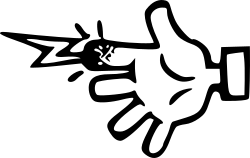
\includegraphics[width=2cm]{sensation}};

\draw (-5.4,1.5) node [left, text width=1cm, align=right] {Non défini};
\draw [->] (-5.2,1.5) -- (-4.5,1.5);
\draw (-4.2,1.5) node [anchor=mid west, text width=7cm] {Seuil de non lâcher, paralysie musculaire};
\draw (3.2,1.5) node [anchor=west] {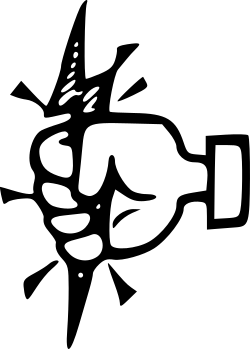
\includegraphics[width=1.5cm]{tetanisation}};

\draw (-5.4,3) node [left] {\SI{130}{\milli\ampere}};
\draw [->] (-5.2,3) -- (-4.5,3);
\draw (-4.2,3) node [anchor=mid west, text width=7cm] {Seuil de fibriliation ventriculaire};
\draw (5.1,3) node {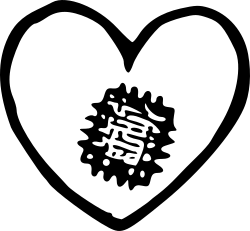
\includegraphics[width=1.5cm]{fibrillation}};

\end{tikzpicture}
\end{figure}

%\end{document}

\begin{itemize}
\item Il est moins difficile de lâcher les parties tenues à la main sous un courant continu\,;
\item Le seuil de fibrillation ventriculaire est plus élevé.
\end{itemize}

\section{Paramètres influençant les risques électriques}

L'intensité de contact $I_c$, la durée de contact $t$, la tension de contact $U_c$ et la résistance du corps humain $R$ sont autant de paramètres à prendre en compte lors de l'évaluation des risques électriques.

\begin{figure}[h]
\caption{Courbe de l'intensité de contact $I_c$ en fonction du temps $t=f(I_c)$\supercite{IEC:60479-2007}\label{graph:intensite_contact_temps}}
\begin{center}
\begin{tikzpicture}

\begin{axis}[
/pgf/number format/.cd, use comma, 1000 sep={\,}, %format numérique européen
axis x line=bottom, axis y line = left,
no markers,
width=\linewidth, height=8cm, %hauteur/largeur
%title={Courbe de l'intensité de contact $I_c$ en fonction du temps $t=f(I_c)$},
grid=major,
enlarge x limits=false, 
xmode=log, xmin=0.1, xmax=6000, xtick={0.1, 0.2, 0.5, 1, 2, 5, 10, 20, 50, 100, 200, 500, 1000, 2000, 5000},
xlabel={Intensité du courant $I_c$ passant dans le corps en \si{\milli\ampere}}, log ticks with fixed point,
ymode=log, ymin=10, ymax=12000, ytick={10, 20, 50, 100, 200, 500, 1000, 2000, 5000, 10000},
ylabel={Durée $t$ du passage du courant en \si{\milli\second}},
]

\path[name path=ha] (0.1,10000) -- (0.5,10000);
\path[name path=la] (0.1,10) -- (0.5,10);
\addplot[YellowGreen, opacity=0.5] fill between[of=la and ha]; %grosse prise de tête pour remplir de couleur entre deux courbes verticales

\addplot [name path=a] (0.5,10) -- (0.5,10000);

\path[name path=ab] (0.5,10) -- (0.5,10000) -- (10.709563224492905,10000);
\addplot [name path=b] table[/pgf/number format/read comma as period]{donnees_courant_duree_b.txt};

\addplot[yellow, opacity=0.5] fill between[of=ab and b];

\addplot [name path=c1, smooth] table[/pgf/number format/read comma as period]{donnees_courant_duree_c1.txt};

\addplot[yellow!75!red, opacity=0.5] fill between[of=b and c1];

\addplot [name path=c2, smooth] table[/pgf/number format/read comma as period]{donnees_courant_duree_c2.txt};

\addplot[yellow!50!red, opacity=0.5] fill between[of= c1 and c2]; %bien inverser le sens d'une des deux listes de données pour que la fonction "fill between" fonctionne correctement

\addplot [name path=c3, smooth] table[/pgf/number format/read comma as period]{donnees_courant_duree_c3.txt};

\addplot[yellow!25!red, opacity=0.5] fill between[of= c2 and c3]; %bien inverser le sens d'une des deux listes de données pour que la fonction "fill between" fonctionne correctement

\path[name path=ec3] (1427.1112552188479, 10) -- (5000,10) -- (5000, 10000);

\addplot[red, opacity=0.5] fill between[of=ec3 and c3];

\end{axis}
\end{tikzpicture}
\end{center}
\end{figure}

\begin{mdframed}
\begin{itemize}
\item[\textcolor{YellowGreen}{\rule{1.5em}{1.2ex}}] Aucune réaction physiologique\,;
\item[\textcolor{yellow}{\rule{1.5em}{1.2ex}}] Aucun effet physiologique dangereux\,;
\item[\textcolor{yellow!75!red}{\rule{1.5em}{1.2ex}}] Aucun dommage corporel. Possibilité de difficultés respiratoires et de contractions musculaires, de troubles réversibles de la formation et de la conduite des impulsions cardiaques (y compris fibrillation des oreillettes et arrêts cardiaques momentanés sans fibrillation ventriculaire ). Phénomènes augmentant proportionnellement avec l'intensité du courant $i_c$ et le temps $t$ d'exposition\,;
\item[\textcolor{yellow!50!red}{\rule{1.5em}{1.2ex}}] Même effets que ceux de la zone \textcolor{yellow!75!red}{\rule{1.5em}{1.2ex}} avec une probabilité de fibrillation ventriculaire augmentant jusqu'à 5\%. Possibilité d'effets physiopathologiques, tels qu'un arrêt cardiaque, un arrêt respiratoire ou des brûlures, augmentant proportionnellement avec l'intensité du courant $i_c$ et le temps $t$ d'exposition\,;
\item[\textcolor{yellow!25!red}{\rule{1.5em}{1.2ex}}] Même effets que ceux de la zone \textcolor{yellow!75!red}{\rule{1.5em}{1.2ex}} avec une probabilité de fibrillation ventriculaire augmentant jusqu'à 50\%. Possibilité d'effets physiopathologiques, tels qu'un arrêt cardiaque, un arrêt respiratoire ou des brûlures, augmentant proportionnellement avec l'intensité du courant $i_c$ et le temps $t$ d'exposition\,;
\item[\textcolor{red}{\rule{1.5em}{1.2ex}}] Même effets que ceux de la zone \textcolor{yellow!75!red}{\rule{1.5em}{1.2ex}} avec une probabilité de fibrillation ventriculaire dépassant 50\%. Possibilité d'effets physiopathologiques, tels qu'un arrêt cardiaque, un arrêt respiratoire ou des brûlures, augmentant proportionnellement avec l'intensité du courant $i_c$ et le temps $t$ d'exposition.
\end{itemize}
\end{mdframed}

Si une personne subit un choc électrique sans en succomber, il s'agit d'une \emph{électrisation}. Si la personne décède suite au choc électrique, il s'agit d'une \emph{électrocution}.

\begin{figure}[H]
\caption{Courbe de la tension de contact $U_c$ en fonction du temps de coupure maximal $t=f(U_c)$\label{graph:tension_contact_temps}}
\begin{center}
\begin{tikzpicture}

\begin{axis}[
/pgf/number format/.cd, use comma, 1000 sep={\,}, %format numérique européen
axis x line=bottom, axis y line = left,
no markers,
width=12cm, height=12cm, %hauteur/largeur
%title={Courbe de la tension de contact $U_c$ en fonction du temps de coupure maximal $t=f(U_c)$},
grid=both,
enlarge x limits=false, 
xmode=log, xmin=10, xmax=600, xtick={10, 20, 30, 50, 100, 200, 300, 500},
xlabel={Tension de contact $U_c$ en \si{\volt}}, log ticks with fixed point,
ymode=log, ymin=0.01, ymax=12, ytick={0.01, 0.02, 0.03, 0.04, 0.05, 1, 0.2, 0.3, 0.4, 0.5, 1, 2, 3, 4, 5, 10},
ylabel={Temps $t$ de coupure maximal en \si\second},
]

\addplot table[/pgf/number format/read comma as period]{donnees_tension_duree_12V.txt};
\addlegendentry{12\si\volt};
\addplot table[/pgf/number format/read comma as period]{donnees_tension_duree_25V.txt};
\addlegendentry{25\si\volt};
\addplot table[/pgf/number format/read comma as period]{donnees_tension_duree_50V.txt};
\addlegendentry{50\si\volt};

\end{axis}
\end{tikzpicture}
\end{center}
\end{figure}

La peau constitue l'isolant contre la pénétration du courant dans le corps humain, et sa résistance électrique varie selon son état de surface et son épaisseur. Pour une peau sèche et fine, on peut estimer que la barrière isolante cède au-delà d'une tension d'environ \SI{50}{\volt}, et le courant pourra dès lors pénétrer de manière plus importante dans le corps humain.\\
En règle générale, on considère la résistance moyenne du corps humain entre \SI{300}{\ohm} et \SI{1000}{\ohm} mais cela peut varier selon les conditions de contact.\supercite{Delahaye2015}

\begin{figure}[H]
\caption{Courbe de la tension de contact $U_c$ en fonction de la résistance du corps humain $R=f(U_c)$\label{graph:tension_contact_resistance}}
\begin{center}
\begin{tikzpicture}

\begin{axis}[
/pgf/number format/.cd, use comma, 1000 sep={\,}, %format numérique européen
axis x line=bottom, axis y line = left,
width=13cm, height=8cm, %hauteur/largeur
%title={Courbe de la tension de contact $U_c$ en fonction de la résistance du corps humain $R=f(U_c)$},
grid=both,
legend cell align={left},
enlarge x limits=false, 
xmin=0, xmax=400, xtick={25, 50, 250, 380},
xlabel={Tension de contact $U_c$ en \si{\volt}},
ymin=0, ymax=6, ytick={1, 2, 3, 4, 5},
ylabel={Résistance du corps humain $R$ en \si{\kilo\ohm}},
]

\addplot [smooth, black] table[/pgf/number format/read comma as period]{donnees_tension_resistance_peauseche.txt};
\addlegendentry{Peau sèche};
\addplot [smooth, brown] table[/pgf/number format/read comma as period]{donnees_tension_resistance_peauhumide.txt};
\addlegendentry{Peau humide};
\addplot [smooth, red] table[/pgf/number format/read comma as period]{donnees_tension_resistance_peaumouillee.txt};
\addlegendentry{Peau mouillée};
\addplot [smooth, blue] table[/pgf/number format/read comma as period]{donnees_tension_resistance_peauimmergee.txt};
\addlegendentry{Peau immergée};
\end{axis}
\end{tikzpicture}
\end{center}
\end{figure}

\section{Nature des contacts}

\subsection{Contact direct}

\subsubsection{Définition}

Contact des personnes avec les parties actives du matériel électrique (pièces ou conducteurs sous tension). La personne rentre en contact direct avec un élément sous tension suite à une négligence ou un non-respect des consignes de sécurité. Dans ce cas, l'électrocution ou l'électrisation sont la conséquence de cette maladresse ou négligence.

\subsubsection{Catégories}

%--------------------------------------
%ELECTROTECHNIQUE - SCHEMA DE LIAISON A LA TERRE
%--------------------------------------

%utiliser les environnement \begin{comment} \end{comment} pour mettre en commentaire le préambule une fois la programmation appelée dans le document maître (!ne pas oublier de mettre en commentaire \end{document}!)

\begin{comment}

\documentclass[a4paper, 11pt, twoside, fleqn]{memoir}

\usepackage{AOCDTF}

%--------------------------------------
%CANEVAS
%--------------------------------------

\newcommand\BoxColor{\ifcase\thechapshift blue!30\or brown!30\or pink!30\or cyan!30\or green!30\or teal!30\or purple!30\or red!30\or olive!30\or orange!30\or lime!30\or gray!\or magenta!30\else yellow!30\fi} %définition de la couleur des marqueurs de chapitre

\newcounter{chapshift} %compteur de chapitre du marqueur de chapitre
\addtocounter{chapshift}{-1}
	
\newif\ifFrame %instruction conditionnelle pour les couleurs des pages
\Frametrue

\pagestyle{plain}

% the main command; the mandatory argument sets the color of the vertical box
\newcommand\ChapFrame{%
\AddEverypageHook{%
\ifFrame
\ifthenelse{\isodd{\value{page}}}
  {\backgroundsetup{contents={%
  \begin{tikzpicture}[overlay,remember picture]
  \node[
  	rounded corners=3pt,
    fill=\BoxColor,
    inner sep=0pt,
    rectangle,
    text width=1.3cm,
    text height=5.5cm,
    align=center,
    anchor=north west
  ] 
  at ($ (current page.north west) + (-0cm,-2*\thechapshift cm) $) %nombre négatif = espacement des marqueurs entre les différents chapitres (à régler en fin de rédaction) (4.5cm vaut un espacement équivalement à la hauteur du marqueur, une page peut en contenir 6 avec cet espacement-la mais il est le plus équilibré)
    {\rotatebox{90}{\hspace*{.3cm}%
      \parbox[c][0.9cm][t]{5cm}{%
        \raggedright\textcolor{black}{\sffamily\textbf{\leftmark}}}}};
  \end{tikzpicture}}}
  }
  {\backgroundsetup{contents={%
  \begin{tikzpicture}[overlay,remember picture]
  \node[
  	rounded corners=3pt,
    fill=\BoxColor,
    inner sep=0pt,
    rectangle,
    text width=1.3cm,
    text height=5.5cm,
    align=center,
    anchor=north east
  ] 
  at ($ (current page.north east) + (-0cm,-2*\thechapshift cm) $) %nombre négatif = espacement des marqueurs entre les différents chapitres (à régler en fin de rédaction) (4.5cm vaut un espacement équivalement à la hauteur du marqueur, une page peut en contenir 6 avec cet espacement-la mais il est le plus équilibré)
    {\rotatebox{90}{\hspace*{.3cm}%
      \parbox[c][0.9cm][t]{5cm}{%
        \raggedright\textcolor{black}{\sffamily\textbf{\leftmark}}}}};
  \end{tikzpicture}}}%
  }
  \BgMaterial%
  \fi%
}%
  \stepcounter{chapshift}
}

\renewcommand\chaptermark[1]{\markboth{\thechapter.~#1}{}} %redéfinition du marqueur de chapitre pour ne contenir que le titre du chapitre %à personnaliser selon le nombre de chapitre dans le cours

%--------------------------------------
%corps du document
%--------------------------------------

\begin{document} %corps du document
	\openleft %début de chapitre à gauche

\end{comment}

\begin{wrapfigure}{R}{0pt} %insertion figure dans texte
\begin{tikzpicture}[circuit ee IEC] 
%\DrawGrid{(-7,-5)}{(7,3)} %grille d'aide pour le placement des objets

\fill [gray!50] (-1,-3) -- (5,-3) -- (5,-3.2) -- (-1,-3.2) -- cycle;
\draw [thick] (-1,-3) -- (5,-3);

\node (V) [voltage source] at (0,0) {}; %schéma électrique
\node (C) [make contact] at (2,0) {};
\node (L) [bulb] at (4,0) {};
\draw [brown] (V) to node {} (C);
\draw [brown] (C) to node {} (L);
\draw [blue] (V) |- (2,0.5);
\draw [blue] (2,0.5) -| (L);

\fill [yellow!, decoration=lightning bolt, decorate] (0.4,-0.8) -- (0.9,0); %éclairs
\fill [yellow!, decoration=lightning bolt, decorate] (2.3,0.5) -- (2.8,1.3);
\path [postaction={on each segment={mid arrow=red}}] (0.9,0) -- (1,-0.2) -- (1.4,-0.6)  -- (2,-1) -- (2.6,-1) -- (2.7,-0.2) -- (2.5,0.3) -- (2.3,0.5);

\draw (2,-1) -- (2.3,-2) -- (2.6,-1) ; %tronc
\draw (2.3,-1) -- (2.3, -0.8); %cou
\draw (2.3,-0.5) circle [radius=0.3cm]; %tête
\draw (0.9,0) -- (1,-0.2) -- (1.4,-0.6)  -- (2,-1) -- (2.6,-1) -- (2.7,-0.2) -- (2.5,0.3) -- (2.3,0.5); %bras
\draw (2.3,-2.93) -- (2.5,-2.9) -- (2.3, -2) -- (1.6,-2.1) -- (1.2,-2.4) -- (1.1,-2.2); %jambes
\filldraw ([shift=(-10:0.3cm)]2.3,-0.5) arc (-10:150:0.3cm); %casquette
\draw (2.04,-0.34) -- ++ (140:0.3cm); 

\end{tikzpicture}
\end{wrapfigure}
%\end{document}



\paragraph{Contact entre deux phases ou la phase et le neutre} 
Contact le moins fréquent mais le plus dangereux car la résistance pied/sol n'intervient pas. La personne qui touche les deux est alors soumise à la tension simple $V$ ou composée $U$ du réseau. La résistance globale du corps devient alors très faible et le courant en est d'autant plus élevé.\\ Dans ce cas, le corps humain se comporte comme un récepteur et aucun appareil de coupure ne peut détecter ce contact comme provoquant un défaut, seule une intervention externe pourra couper le courant.\\

Si la personne est soumise à une tension de contact $U_c$ de \SI{230}{\volt} et que l'on estime la résistance résultante $R$ des résistance main/fil + résistance des bras à environ \SI{1,5}{\kilo\ohm}, on peut calculer l'intensité du courant traversant le corps comme suit :

\begin{align*}
I 	&= \frac{U_c}{R} \\
	&= \frac{230}{1500} \\
	&= \SI{150}{\milli\ampere}
\end{align*}

En se référençant au tableau \superref{graph:intensite_contact_temps}, on peut constater que le temps de réaction de coupure (venant d'une intervention externe) doit être très court. Effectivement, après une seconde, le risque de fibrillation ventriculaire dépasse déjà les 50\%, ce qui augmente sensiblement le risque d'arrêt cardiaque.

%--------------------------------------
%ELECTROTECHNIQUE - SCHEMA DE LIAISON A LA TERRE
%--------------------------------------

%utiliser les environnement \begin{comment} \end{comment} pour mettre en commentaire le préambule une fois la programmation appelée dans le document maître (!ne pas oublier de mettre en commentaire \end{document}!)

\begin{comment}

\documentclass[a4paper, 11pt, twoside, fleqn]{memoir}

\usepackage{AOCDTF}

%--------------------------------------
%CANEVAS
%--------------------------------------

\newcommand\BoxColor{\ifcase\thechapshift blue!30\or brown!30\or pink!30\or cyan!30\or green!30\or teal!30\or purple!30\or red!30\or olive!30\or orange!30\or lime!30\or gray!\or magenta!30\else yellow!30\fi} %définition de la couleur des marqueurs de chapitre

\newcounter{chapshift} %compteur de chapitre du marqueur de chapitre
\addtocounter{chapshift}{-1}
	
\newif\ifFrame %instruction conditionnelle pour les couleurs des pages
\Frametrue

\pagestyle{plain}

% the main command; the mandatory argument sets the color of the vertical box
\newcommand\ChapFrame{%
\AddEverypageHook{%
\ifFrame
\ifthenelse{\isodd{\value{page}}}
  {\backgroundsetup{contents={%
  \begin{tikzpicture}[overlay,remember picture]
  \node[
  	rounded corners=3pt,
    fill=\BoxColor,
    inner sep=0pt,
    rectangle,
    text width=1.3cm,
    text height=5.5cm,
    align=center,
    anchor=north west
  ] 
  at ($ (current page.north west) + (-0cm,-2*\thechapshift cm) $) %nombre négatif = espacement des marqueurs entre les différents chapitres (à régler en fin de rédaction) (4.5cm vaut un espacement équivalement à la hauteur du marqueur, une page peut en contenir 6 avec cet espacement-la mais il est le plus équilibré)
    {\rotatebox{90}{\hspace*{.3cm}%
      \parbox[c][0.9cm][t]{5cm}{%
        \raggedright\textcolor{black}{\sffamily\textbf{\leftmark}}}}};
  \end{tikzpicture}}}
  }
  {\backgroundsetup{contents={%
  \begin{tikzpicture}[overlay,remember picture]
  \node[
  	rounded corners=3pt,
    fill=\BoxColor,
    inner sep=0pt,
    rectangle,
    text width=1.3cm,
    text height=5.5cm,
    align=center,
    anchor=north east
  ] 
  at ($ (current page.north east) + (-0cm,-2*\thechapshift cm) $) %nombre négatif = espacement des marqueurs entre les différents chapitres (à régler en fin de rédaction) (4.5cm vaut un espacement équivalement à la hauteur du marqueur, une page peut en contenir 6 avec cet espacement-la mais il est le plus équilibré)
    {\rotatebox{90}{\hspace*{.3cm}%
      \parbox[c][0.9cm][t]{5cm}{%
        \raggedright\textcolor{black}{\sffamily\textbf{\leftmark}}}}};
  \end{tikzpicture}}}%
  }
  \BgMaterial%
  \fi%
}%
  \stepcounter{chapshift}
}

\renewcommand\chaptermark[1]{\markboth{\thechapter.~#1}{}} %redéfinition du marqueur de chapitre pour ne contenir que le titre du chapitre %à personnaliser selon le nombre de chapitre dans le cours

%--------------------------------------
%corps du document
%--------------------------------------

\begin{document} %corps du document
	\openleft %début de chapitre à gauche

\end{comment}

\begin{wrapfigure}{R}{0pt} %insertion figure dans texte
\begin{tikzpicture}[circuit ee IEC] 
%\DrawGrid{(-7,-5)}{(7,3)} %grille d'aide pour le placement des objets

\fill [gray!50] (-1,-3) -- (5,-3) -- (5,-3.2) -- (-1,-3.2) -- cycle;
\draw [thick] (-1,-3) -- (5,-3);

\node (V) [voltage source] at (0,0) {}; %schéma électrique
\node (C) [make contact] at (2,0) {};
\node (L) [bulb] at (4,0) {};
\draw [brown] (V) to node {} (C);
\draw [brown] (C) to node {} (L);
\draw [blue] (V) |- (2,0.5);
\draw [blue] (2,0.5) -| (L);

\fill [yellow!, decoration=lightning bolt, decorate] (0.4,-0.8) -- (0.9,0); %éclairs
\path [postaction={on each segment={mid arrow=red}}] (0.9,0) -- (1,-0.2) -- (1.4,-0.6)  -- (2,-1) -- (2.3,-2) -- (2.5,-2.9) -- (2.5,-3.1) -- (4,-3.1) -- (4,-3.4);

\draw (2,-1) -- (2.3,-2) -- (2.6,-1) ; %tronc
\draw (2.3,-1) -- (2.3, -0.8); %cou
\draw (2.3,-0.5) circle [radius=0.3cm]; %tête
\draw (0.9,0) -- (1,-0.2) -- (1.4,-0.6)  -- (2,-1) -- (2.6,-1) -- (3.2,-1.4) -- (3.4,-2) -- (3.6,-2); %bras
\draw (2.3,-2.93) -- (2.5,-2.9) -- (2.3, -2) -- (1.6,-2.1) -- (1.2,-2.4) -- (1.1,-2.2); %jambes
\filldraw ([shift=(-10:0.3cm)]2.3,-0.5) arc (-10:150:0.3cm); %casquette
\draw (2.04,-0.34) -- ++ (140:0.3cm); 

\end{tikzpicture}
\end{wrapfigure}

%\end{document}



\paragraph{Contact entre la phase et la terre}
Contact relativement plus fréquent et moins dangereux que le précédent car la résistance pied/sol et la détection de courant de fuite interviennent. Ce contact direct est rendu possible lorsque le neutre est relié à la terre (\emph{régime TT} et \emph{régime TN}) et soumet la personne à la tension simple $V$ du réseau.\\
La résistance pied/sol augmente donc la résistante résultante $R$ comprenant donc la résistance main/fil + résistance des bras + résistance pied/sol. Si l'on estime cette résistance à \SI{16}{\kilo\ohm} et que l'on conserve la tension de contact $U_c$ de \SI{230}{\volt}, on peut calculer l'intensité du courant traversant le corps comme suit :

\begin{align*}
I 	&= \frac{U_c}{R} \\
	&= \frac{230}{16000} \\
	&= \SI{14,4}{\milli\ampere}
\end{align*}

En se référençant au tableau \superref{graph:intensite_contact_temps}, on peut constater cette fois-ci que la situation présente moins de danger que précédemment si le contact ne dépasse toutefois pas les deux secondes. Cette résistance dépend évidement de la nature des semelles, et dans le cas où la personne serait pied nu, la résistance pied/sol baissera au point de considérer le contact comme un contact phase/neutre.\\

Dans cette configuration-là, le corps entraine également une fuite du courant électrique vers la terre. Cette spécificité est exploité par un appareil de protection dédié à la détection de fuite de courant, le dispositifs différentiel résiduel (DDR), ou différentiel.

\subsubsection{Protection contre les contacts directs}

\begin{table}[H]
\caption{Moyen de protection contre les contacts directs\label{tab:protection_contact_direct}}
\begin{threeparttable} %note dans tableau
\begin{tabularx}{\textwidth}{p{4cm}XX}
\toprule
\thead{Catégorie}																	& \thead{Principe}																																& \thead{Moyen} \\
\midrule
Contact phase/neutre																& Mise hors de portée des pièce sous tensions																							& 
\begin{tabitemize}
\item Capotage, isolement, mise sous enveloppe\ldots\,;
\item Respect de l'indice de protection (IP) minimal\tnote{1}.
\end{tabitemize} \\
																							&	Utilisation d'une tension non dangereuse																							&	Alimentation des circuits en TBT\tnote{2} \\
\addlinespace
Contact phase/neutre et phase/terre										&	Isolement par rapport au réseau TT																										& Transformateur d'isolement\tnote{3} \\
																							&	Contrôle du courant de fuite $I_f$ (ne devant pas dépasser quelques dizaines de \si{\milli\ampere}		& DDR de basse sensibilité (\SI{10}{\milli\ampere} ou \SI{30}{\milli\ampere}\tnote{4}\\
\bottomrule
\end{tabularx}
\begin{tablenotes}
    \item[1] Informations complémentaires sur les IP en \superref{subsec:indice_protection}\,;
    \item[2] Informations complémentaires sur les différentes TBT en \superref{subsec:TBT} \,;
    \item[3] Informations complémentaires sur le transformateur d'isolement en \superref{subsec:transformateur_isolement} \,;
    \item[4] Détails sur le DDR en .
\end{tablenotes}
\end{threeparttable}
\end{table}

\subsection{Contact indirect}

\subsubsection{Définition}

\begin{description}
\item[Contact indirect] Contact des personnes avec les masses métalliques mises accidentellement sous tension, généralement suite à un défaut d'isolement (déconnexion des fils, vieillissement ou rupture des isolants\ldots). Dans ce cas, la responsabilité de la personne n'est pas mise en jeu et l'électrisation (et électrocution) est la conséquence d'un défaut imprévisible.
\item[Masse] Partie conductrice susceptible d'être touchée et manipulée par une personne et normalement isolée des éléments sous tension, qui peut toutefois être accidentellement portée à un potentiel dangereux.
\end{description}

\subsubsection{Principe}

%--------------------------------------
%ELECTROTECHNIQUE - SCHEMA DE LIAISON A LA TERRE
%--------------------------------------

%utiliser les environnement \begin{comment} \end{comment} pour mettre en commentaire le préambule une fois la programmation appelée dans le document maître (!ne pas oublier de mettre en commentaire \end{document}!)

\begin{comment}

\documentclass[a4paper, 11pt, twoside, fleqn]{memoir}

\usepackage{AOCDTF}

%--------------------------------------
%CANEVAS
%--------------------------------------

\newcommand\BoxColor{\ifcase\thechapshift blue!30\or brown!30\or pink!30\or cyan!30\or green!30\or teal!30\or purple!30\or red!30\or olive!30\or orange!30\or lime!30\or gray!\or magenta!30\else yellow!30\fi} %définition de la couleur des marqueurs de chapitre

\newcounter{chapshift} %compteur de chapitre du marqueur de chapitre
\addtocounter{chapshift}{-1}
	
\newif\ifFrame %instruction conditionnelle pour les couleurs des pages
\Frametrue

\pagestyle{plain}

% the main command; the mandatory argument sets the color of the vertical box
\newcommand\ChapFrame{%
\AddEverypageHook{%
\ifFrame
\ifthenelse{\isodd{\value{page}}}
  {\backgroundsetup{contents={%
  \begin{tikzpicture}[overlay,remember picture]
  \node[
  	rounded corners=3pt,
    fill=\BoxColor,
    inner sep=0pt,
    rectangle,
    text width=1.3cm,
    text height=5.5cm,
    align=center,
    anchor=north west
  ] 
  at ($ (current page.north west) + (-0cm,-2*\thechapshift cm) $) %nombre négatif = espacement des marqueurs entre les différents chapitres (à régler en fin de rédaction) (4.5cm vaut un espacement équivalement à la hauteur du marqueur, une page peut en contenir 6 avec cet espacement-la mais il est le plus équilibré)
    {\rotatebox{90}{\hspace*{.3cm}%
      \parbox[c][0.9cm][t]{5cm}{%
        \raggedright\textcolor{black}{\sffamily\textbf{\leftmark}}}}};
  \end{tikzpicture}}}
  }
  {\backgroundsetup{contents={%
  \begin{tikzpicture}[overlay,remember picture]
  \node[
  	rounded corners=3pt,
    fill=\BoxColor,
    inner sep=0pt,
    rectangle,
    text width=1.3cm,
    text height=5.5cm,
    align=center,
    anchor=north east
  ] 
  at ($ (current page.north east) + (-0cm,-2*\thechapshift cm) $) %nombre négatif = espacement des marqueurs entre les différents chapitres (à régler en fin de rédaction) (4.5cm vaut un espacement équivalement à la hauteur du marqueur, une page peut en contenir 6 avec cet espacement-la mais il est le plus équilibré)
    {\rotatebox{90}{\hspace*{.3cm}%
      \parbox[c][0.9cm][t]{5cm}{%
        \raggedright\textcolor{black}{\sffamily\textbf{\leftmark}}}}};
  \end{tikzpicture}}}%
  }
  \BgMaterial%
  \fi%
}%
  \stepcounter{chapshift}
}

\renewcommand\chaptermark[1]{\markboth{\thechapter.~#1}{}} %redéfinition du marqueur de chapitre pour ne contenir que le titre du chapitre %à personnaliser selon le nombre de chapitre dans le cours

%--------------------------------------
%corps du document
%--------------------------------------

\begin{document} %corps du document
	\openleft %début de chapitre à gauche

\end{comment}

\begin{wrapfigure}{R}{0pt} %insertion figure dans texte
\begin{tikzpicture}[circuit ee IEC] 
%\DrawGrid{(-2,-5)}{(7,1)} %grille d'aide pour le placement des objets

\fill [gray!50] (-1,-3) -- (5,-3) -- (5,-3.2) -- (-1,-3.2) -- cycle;
\draw [thick] (-1,-3) -- (5,-3);

\node (V) [voltage source] at (0,0) {}; %schéma électrique
\node (L) [bulb] at (4,0) {};
\node (B) [contact] at (4,-0.4) {};
\node (R) [resistor, point down, info=$R_t$, tiny circuit symbols] at (4,-2) {};
\node (G) [ground, point down] at (4,-3.5) {};
\draw [brown] (V) to node {} (L);
\draw [green!] (B) to node {} (R) ; 
\draw [green!] (R) to node {} (G) ; 
\draw [dashed, yellow!] (B) to node {} (R) ;
\draw [dashed, yellow!] (R) to node {} (G) ;
\draw [blue] (V) |- (2,0.5);
\draw [blue] (2,0.5) -| (L);
\draw (3.6,-0.4) rectangle (4.4,0.4);

\fill [yellow!, decoration=lightning bolt, decorate] (3.6,0) -- (3.1,0.8); %éclairs
\fill [yellow!, decoration=lightning bolt, decorate] (3.6,-0.2) -- (3.3,-1.1);
\path [postaction={on each segment={mid arrow=red}}] (3.6,-0.2) -- (3.4,-0.4) --  (2.6,-1) -- (2.3,-2) -- (2.1,-2.9) -- (2.3,-2.96) -- (4,-3.1);
\path [postaction={on each segment={mid arrow=red}}] (3.6,-0.4) -- (4,-0.4) -- (4,-1.6);
\path [postaction={on each segment={mid arrow=red}}] (4,-2.4) -- (4,-3) -- (4,-3.4);


\draw (2,-1) -- (2.3,-2) -- (2.6,-1) ; %tronc
\draw (2.3,-1) -- (2.3, -0.8); %cou
\draw (2.3,-0.5) circle [radius=0.3cm]; %tête
\filldraw ([shift=(190:0.3cm)]2.3,-0.5) arc (190:30:0.3cm); %casquette
\draw (0.9,-1.6) -- (1,-1.8) -- (1.4,-1.4)  -- (2,-1) -- (2.6,-1)  -- (3.4,-0.4) -- (3.6,-0.2); %bras
\draw (2.3,-2.96) -- (2.1,-2.9) -- (2.3,-2) -- (3.1,-2.1) -- (3.4,-2.6) -- (3.5,-2.4); %jambes
\draw (2.55,-0.34) -- ++ (40:0.3cm); 

\end{tikzpicture}
\end{wrapfigure}

%\end{document}



Ce type de contact peut apparaitre lorsque le neutre est relié à la terre (\emph{régime TT} et \emph{régime TN}) et qu'une masse métallique est mise accidentellement sous tension. Si cette masse est reliée à la terre, un courant de fuite $I_f$ va faire son apparition et sera potentiellement détecté par un DDR selon sa sensibilité, si celui-ci est présent et fonctionnel. \`A cause de la résistance de la prise de terre $R_t$, le courant de fuite $I_f$ et le potentiel des masses métalliques augmenteront progressivement avec le temps.\\

Le risque devient de plus en plus élevé, d'autant que le contact indirect est accidentel et les masses métalliques généralement manipulées franchement. \`A cela s'ajoute le fait que les conditions de contact peuvent également être défavorables (zones humides, pieds nus...), ce qui peut augmenter dangereusement l'intensité du courant traversant le corps.

\subsubsection{Protection contre les contacts indirects}

Il existe différents moyens de protections contre les contacts indirects qui varient selon les \emph{schémas de liaison à la terre} (SLT), qui seront détaillé en \superref{chap2:schémas_liaison_terre}. Le principal moyen pour ce faire en régime TT et TN est d'installer un DDR, associé obligatoirement à une \emph{prise de terre} du transformateur de l'installation électrique et une \emph{mise à la terre} (MALT) des matériels et structures conducteurs susceptibles d'être accidentellement mis sous tension. Ces deux spécificités de l'installation électrique permettront au courant de s'échapper vers la terre via la mise à la terre et former une boucle jusqu'à la prise de terre. Cela formera une boucle de \emph{courant de défaut} $I_d$ qui sera détecté par le DDR, qui, selon le type de protection exigé, jouera un rôle de protection des personne (signalement de défaut et/ou sectionnement de l'installation en défaut).\\
En régime IT, la protection contre les contacts indirects s'effectue de manière similaire mais supervisée par un service technique.\\

L'usage d'appareils électriques de classe II ou III est également un autre moyen de protection contre les contacts indirects. Plus de détails sur ces différentes solutions en \superref{sec:moyens_protection_contacts_indirects}. 

%\end{document}


	%--------------------------------------
	%style des annexes
	%--------------------------------------

	\appendix %appel des annexes
	\clearpage\Framefalse %défini la booléenne Frame comme false -> pas de marqueurs de chapitre
	\openany
	%\thispagestyle{empty}\null\clearpage %force la page titre des annexes à s'afficher sur la droite si ça n'est pas le cas
	\appendixpage
	\openleft

	%--------------------------------------
	%inclusion des chapitres
	%--------------------------------------

	%--------------------------------------
%ELECTROTECHNIQUE - SCHEMA DE LIAISON A LA TERRE
%--------------------------------------

%utiliser les environnement \begin{comment} \end{comment} pour mettre en commentaire le préambule une fois la programmation appelée dans le document maître (!ne pas oublier de mettre en commentaire \end{document}!)

%\begin{comment}

\documentclass[a4paper, 11pt, twoside, fleqn]{memoir}

\usepackage{AOCDTF}

%--------------------------------------
%CANEVAS
%--------------------------------------

\newcommand\BoxColor{\ifcase\thechapshift blue!30\or brown!30\or pink!30\or cyan!30\or green!30\or teal!30\or purple!30\or red!30\or olive!30\or orange!30\or lime!30\or gray!\or magenta!30\else yellow!30\fi} %définition de la couleur des marqueurs de chapitre

\newcounter{chapshift} %compteur de chapitre du marqueur de chapitre
\addtocounter{chapshift}{-1}
	
\newif\ifFrame %instruction conditionnelle pour les couleurs des pages
\Frametrue

\pagestyle{plain}

% the main command; the mandatory argument sets the color of the vertical box
\newcommand\ChapFrame{%
\AddEverypageHook{%
\ifFrame
\ifthenelse{\isodd{\value{page}}}
  {\backgroundsetup{contents={%
  \begin{tikzpicture}[overlay,remember picture]
  \node[
  	rounded corners=3pt,
    fill=\BoxColor,
    inner sep=0pt,
    rectangle,
    text width=1.3cm,
    text height=5.5cm,
    align=center,
    anchor=north west
  ] 
  at ($ (current page.north west) + (-0cm,-2*\thechapshift cm) $) %nombre négatif = espacement des marqueurs entre les différents chapitres (à régler en fin de rédaction) (4.5cm vaut un espacement équivalement à la hauteur du marqueur, une page peut en contenir 6 avec cet espacement-la mais il est le plus équilibré)
    {\rotatebox{90}{\hspace*{.3cm}%
      \parbox[c][0.9cm][t]{5cm}{%
        \raggedright\textcolor{black}{\sffamily\textbf{\leftmark}}}}};
  \end{tikzpicture}}}
  }
  {\backgroundsetup{contents={%
  \begin{tikzpicture}[overlay,remember picture]
  \node[
  	rounded corners=3pt,
    fill=\BoxColor,
    inner sep=0pt,
    rectangle,
    text width=1.3cm,
    text height=5.5cm,
    align=center,
    anchor=north east
  ] 
  at ($ (current page.north east) + (-0cm,-2*\thechapshift cm) $) %nombre négatif = espacement des marqueurs entre les différents chapitres (à régler en fin de rédaction) (4.5cm vaut un espacement équivalement à la hauteur du marqueur, une page peut en contenir 6 avec cet espacement-la mais il est le plus équilibré)
    {\rotatebox{90}{\hspace*{.3cm}%
      \parbox[c][0.9cm][t]{5cm}{%
        \raggedright\textcolor{black}{\sffamily\textbf{\leftmark}}}}};
  \end{tikzpicture}}}%
  }
  \BgMaterial%
  \fi%
}%
  \stepcounter{chapshift}
}

\renewcommand\chaptermark[1]{\markboth{\thechapter.~#1}{}} %redéfinition du marqueur de chapitre pour ne contenir que le titre du chapitre %à personnaliser selon le nombre de chapitre dans le cours

%--------------------------------------
%corps du document
%--------------------------------------

\begin{document} %corps du document
	\openleft %début de chapitre à gauche

%\end{comment}

\chapter{Informations complémentaires sur les dangers de l'électricité}

Cette annexe regroupe des données complémentaires mentionnées dans le \superref{chap:dangers_electricite}. Il n'est pas nécessaire de les retenir par c\oe{}ur mais ces informations constituent un support appréciable pour toute précision concernant ce chapitre.

\section{\'Etat des lieux de la prévention des risques électriques\label{sec:etat_lieux_prevention_electrique}}

\section{Statistiques}

\subsection{Accidents d'origine électrique}

Les accidents du travail d'origine électrique diminuent depuis la mise en place du décret du 14 novembre 1962 qui attrait à la protection des travailleurs contre les dangers de l'électricité. Entre 1962 et 2000, le nombre d'incidents a baissé de 74\%. 

\begin{center}
\begin{tikzpicture}
\begin{axis}[
/pgf/number format/.cd, use comma, 1000 sep={\,}, %format numérique européen
date coordinates in=x,
axis x line=bottom, axis y line = left,
xmin=1975-01-01,
xmax=2005-12-31,
ymin=0,
ymax=3100,
legend cell align={left},
no markers,
grid=major,
ytick={0, 500, 1000, 1500, 2000, 2500, 3000},
xtick={1975-01-01, 1980-01-01, 1985-01-01, 1990-01-01, 1995-01-01, 2000-01-01, 2005-01-01},
title={Variation du nombre d'accidents du travail d'origine électrique},
height=8cm,width=\linewidth,
ylabel={Nombre d'accidents},
legend entries={Accidents avec arrêt, Accidents graves, Accidents mortels},
xticklabel={\year},
]

\addplot[mark=none]table{donnees_accident_arret.txt};
\addlegendentry{Accidents avec arrêt};
\addplot[mark=none, red]table{donnees_accident_grave.txt};
\addlegendentry{Accidents graves};
\addplot[mark=none, blue]table{donnees_accident_mortel.txt};
\addlegendentry{Accidents mortels};
\end{axis}
\end{tikzpicture}
\end{center}

\subsection{Secteurs les plus atteints}

Durant l'année 2008, on dénombrait 771 accidents d'origine électrique. Les secteurs les plus touchés sont : 
\begin{description}
\item[30\% :] bâtiment et travaux publics,\;
\item[17\% :] métallurgie,\;
\item[16\% :] service et travail temporaire,\;
\item[11\% :] alimentation.
\end{description}

\subsection{Facteurs principaux}

Les principaux facteurs ayant causé l'accident sont :
\begin{description}
\item[31\% :] mode opératoire inapproprié ou dangereux\,;
\item[15\% :] application incomplète\,;
\item[12\% :] formation insuffisante\,;
\item[12\% :] état du matériel\,;
\item[11\% :] état du sol.
\end{description}

\subsection{Type de contact}

\begin{description}
\item[75\% :] contact direct\,;
\item[20\% :] contact indirect\,;
\item[5\% :] non précisé.
\end{description}

\subsection{Type de dommages}

Ces statistiques sur plusieurs années sont relativement constantes. Elles précisent que :
\begin{description}
\item[60\% :] brûlures\,;
\item[$\approx$ 33\% :] localisation multiples (les yeux, les membres supérieurs et les mains sont les plus touchés)\,;
\item[5\% :] lésions internes.
\end{description}

\subsection{Conclusion}

On peut conclure de ces statistiques que depuis une trentaine d'années, le nombre d'accidents dus à l'électricité :
\begin{itemize}
\item diminue régulièrement\,;
\item demeurent particulièrement graves.
\end{itemize}

Le risque d'accidents est certe mieux maitrisé qu'auparavant mais il reste toujours présent.

\section{Différents effets du courant électriques\label{sec:effet_courant_électrique}}

\subsection{Effet thermique}

Il est admis que les brûlures électriques peuvent apparaitre à des intensités relativement faibles ($\approx \SI{10}{\milli\ampere}$), si le contact est maintenu quelques minutes

\subsection{Effet tétanisant}

Lorsque la tension est alternatif, les muscles se situant sur le trajet du courant électrique se contractent. Cet effet, surtout s'il s'agit des muscles de la main, peuvent empêcher tout dégagement volontaire de la victime. Pour l'extraire de cette situation, il convient de stopper le contact crispé en la poussant à l'aide d'un objet non conducteur.

\subsection{Effets respiratoires et circulatoires}

Les muscles respiratoires pouvant également être crispés par le courant, il suffit de \SI{60}{\second} pour bloquer la respiration. Cela provoque une asphyxie, appelée également \emph{syncope blanche}.\\
Une fibrillation ventriculaire se manifeste également pour les mêmes ordres de grandeurs. C'est le résultat de la contraction anarchiques des fibrilles du muscle cardiaque. Ces battements du c\oe{}ur rapides et désordonnés ne permettent plus d'assurer une circulation sanguine adéquate et provoque ainsi une syncope cardiaque, appelée aussi \emph{syncope blanche}. Une défibrillation devient indispensable pour stopper cet effet du courant.\\
Au-delà d'un \SI{1}{\ampere}, le courant entraîne un arrêt cardiaque par asystolie, une absence de battements cardiaques sur laquelle une défibrillation n'est pas recommandée.\\
Les lésions cardiaques diffèrent selon certain paramètres, ces information peuvent aider les premiers secours à axer leurs interventions en situation d'extrême urgence : 
\begin{description}
\item[basse tension :] effet excito-moteur et fibrillation ventriculaire\,;
\item[haute tension :] effet joule et asystolie\,;
\item[foudre :] sidération myocardique (dysfonction des contractions du c\oe{}ur difficilement prise en charge).
\end{description}

Lors de la prise en charge d'un patient électrisé, il convient de bien suivre celui-ci sur plusieurs jours car les risques de malaises cardiaques dûs au choc électrique peuvent ressurgir durant une période plus ou moins longue selon les conditions d'électrisation.

\section{Descriptifs des moyens de protections contre les contacts directs}

Les différents moyens de protections sont ici décrits en profondeur à titre informatif.

\subsection{Très basse tension\label{subsec:TBT}}

Il existe trois types de TBT selon la classification du lieux et la nature du courant.

\subsubsection{Principe}

\paragraph{Très Basse Tension de Sécurité (ou Séparation)} Alimentation basse tension ou il n'existe aucun point commun entre le primaire et le secondaire du transformateur, utilisée pour alimenter des appareillages situés dans des locaux humides.
\paragraph{Très Basse Tension de Protection} Alimentation basse tension ou il existe un point commun entre le commun du secondaire et le conducteur de protection, utilisée pour alimenter des machines-outils et automatisme. La liaison du commun au conducteur de protection du secondaire permet d'éviter les mises en marche intempestives pouvant survenir après deux défauts de masse consécutifs dans une commande de machine (alimentation possible d'une bobine de contacteur via la carcasse de l'armoire de commande).
\paragraph{Très Basse Tension Fonctionnelle} Alimentation basse tension ou il existe plusieurs point commun entre le primaire et le secondaire du transformateur (autotransformateur), utilisée pour alimenter des appareillages ne requérant pas d'exigences de sécurité autre qu'une tension nominale de fonctionnement spécifique.

\subsubsection{Architecture}

%--------------------------------------
%ELECTROTECHNIQUE - SCHEMA DE LIAISON A LA TERRE
%--------------------------------------

%utiliser les environnement \begin{comment} \end{comment} pour mettre en commentaire le préambule une fois la programmation appelée dans le document maître (!ne pas oublier de mettre en commentaire \end{document}!)

\begin{comment}

\documentclass[a4paper, 11pt, twoside, fleqn]{memoir}

\usepackage{AOCDTF}

%--------------------------------------
%CANEVAS
%--------------------------------------

\newcommand\BoxColor{\ifcase\thechapshift blue!30\or brown!30\or pink!30\or cyan!30\or green!30\or teal!30\or purple!30\or red!30\or olive!30\or orange!30\or lime!30\or gray!\or magenta!30\else yellow!30\fi} %définition de la couleur des marqueurs de chapitre

\newcounter{chapshift} %compteur de chapitre du marqueur de chapitre
\addtocounter{chapshift}{-1}
	
\newif\ifFrame %instruction conditionnelle pour les couleurs des pages
\Frametrue

\pagestyle{plain}

% the main command; the mandatory argument sets the color of the vertical box
\newcommand\ChapFrame{%
\AddEverypageHook{%
\ifFrame
\ifthenelse{\isodd{\value{page}}}
  {\backgroundsetup{contents={%
  \begin{tikzpicture}[overlay,remember picture]
  \node[
  	rounded corners=3pt,
    fill=\BoxColor,
    inner sep=0pt,
    rectangle,
    text width=1.3cm,
    text height=5.5cm,
    align=center,
    anchor=north west
  ] 
  at ($ (current page.north west) + (-0cm,-2*\thechapshift cm) $) %nombre négatif = espacement des marqueurs entre les différents chapitres (à régler en fin de rédaction) (4.5cm vaut un espacement équivalement à la hauteur du marqueur, une page peut en contenir 6 avec cet espacement-la mais il est le plus équilibré)
    {\rotatebox{90}{\hspace*{.3cm}%
      \parbox[c][0.9cm][t]{5cm}{%
        \raggedright\textcolor{black}{\sffamily\textbf{\leftmark}}}}};
  \end{tikzpicture}}}
  }
  {\backgroundsetup{contents={%
  \begin{tikzpicture}[overlay,remember picture]
  \node[
  	rounded corners=3pt,
    fill=\BoxColor,
    inner sep=0pt,
    rectangle,
    text width=1.3cm,
    text height=5.5cm,
    align=center,
    anchor=north east
  ] 
  at ($ (current page.north east) + (-0cm,-2*\thechapshift cm) $) %nombre négatif = espacement des marqueurs entre les différents chapitres (à régler en fin de rédaction) (4.5cm vaut un espacement équivalement à la hauteur du marqueur, une page peut en contenir 6 avec cet espacement-la mais il est le plus équilibré)
    {\rotatebox{90}{\hspace*{.3cm}%
      \parbox[c][0.9cm][t]{5cm}{%
        \raggedright\textcolor{black}{\sffamily\textbf{\leftmark}}}}};
  \end{tikzpicture}}}%
  }
  \BgMaterial%
  \fi%
}%
  \stepcounter{chapshift}
}

\renewcommand\chaptermark[1]{\markboth{\thechapter.~#1}{}} %redéfinition du marqueur de chapitre pour ne contenir que le titre du chapitre %à personnaliser selon le nombre de chapitre dans le cours

%--------------------------------------
%corps du document
%--------------------------------------

\begin{document} %corps du document
	\openleft %début de chapitre à gauche

\end{comment}

\begin{landscape}
\begin{table}
\caption{Types de Très Basse Tension\label{tab:type_TBT}}
\begin{tabularx}{\linewidth}{p{3,5cm} X p{3cm} p{3,5cm} p{3,5cm} p{3,5cm} p{2cm}}
\toprule
\thead{Domaine \\de tension}		& \thead{Alimentation}			& \thead{Liaison à\\ la terre}			& \thead{Sectionnement et\\protection contre\\ les court-circuits}		& \thead{Protection contre \\ les contacts\\ indirects}		& \thead{Protection contre\\ les contacts\\ directs}				& \thead{Récepteur} \\
\midrule
TBTS (Très Basse Tension de Sécurité)		& Transformateur de sécurité conforme à la norme NF C 52 742		& \makecell[c]{Interdite}		& De tous des conducteurs actifs		& \makecell[c]{Non}		& \makecell[c]{Non} 	& \\
\addlinespace

															& \multicolumn{6}{l}{%
\begin{circuitikz}[circuit ee IEC relay]
%\DrawGrid{(0,-0.5)}{(21,0.5)} %grille d'aide pour le placement des objets
\draw (20.5,0) node[draw](Z){Z};
\draw (Z.west) node[circ, left](E){};
\draw (0,0) to[oosourcetrans, l=classe II] (3,0)
to[make contact={point left, circuit breaker={point left}, thick, name=dis}] (16,0)
to (E);
\draw [thick] (1.7,0.4) arc (90:-90:0.4) -- (0.9,-0.4) -- (0.9,0.4) -- (1.7,0.4);
\draw [thick] (1.5,0.3) -- (1.5,-0.3);
\end{circuitikz}} \\
\addlinespace[1cm]

TBTP (Très Basse Tension de Protection)		& Transformateur de sécurité conforme à la norme NF C 52 742		&  Conducteur actif relié à la terre		& De tous des conducteurs actifs		& \makecell[c]{Non}		& \makecell[c]{Non} 	& \\
\addlinespace
															& \multicolumn{6}{l}{%
\begin{circuitikz}[circuit ee IEC relay]
%\DrawGrid{(0,-0.5)}{(21,0.5)} %grille d'aide pour le placement des objets
\draw (20.5,0) node[draw](Z){Z};
\draw (Z.west) node[circ, left](E){};
\draw (0,0) to[oosourcetrans, l=classe I] (3,0)
to node[circ](C){} (8,0)
to[make contact={point left, circuit breaker={point left}, thick, name=dis}] (11,0)
to (E);
\draw (C) -- (5.5,-1) node[pground]{};
\draw [thick] (1.5,0.3) -- (1.5,-0.3);
\end{circuitikz}} \\
\addlinespace[1cm]

TBTF (Très Basse Tension de Fonctionnelle)		& Transformateur de sécurité d'origine indéterminée		&  Conducteur actif relié à la terre		& De tous des conducteurs actifs		& \makecell[c]{Oui (DDR)}		& \makecell[c]{Oui (appareil IP2X)} 	& \\
\addlinespace
															& \multicolumn{6}{l}{%
\begin{circuitikz}[circuit ee IEC relay]
%\DrawGrid{(0,-0.5)}{(21,0.5)} %grille d'aide pour le placement des objets
\draw (19.5,0) node[draw](Z){Z};
\draw (Z.west) node[circ, left](E){};
\draw (Z.east) node[circ, right](F){};
\draw [rounded corners] (F) -| (20.5,-1) node [tlground]{};
\draw (0,0) to[oosourcetrans] (3,0)
to node[circ](C){} (8,0)
to[make contact={point left, circuit breaker={point left}, thick, name=dis}] (11,0)
to node[iloopshape, rotate=180](D){} (16,0)
to (E);
\draw [dashed, rounded corners] (dis.mid) to (9.5,-1) -- (13.5,-1) to (D.i);
\draw (C) -- (5.5,-1) node[pground]{} ;
\end{circuitikz}} \\
\addlinespace[1cm]

\bottomrule
\end{tabularx}

\end{table}

\end{landscape}

%\end{document}



\subsection{Indice de protection\label{subsec:indice_protection}}

L'indice de protection (IP) est composé de deux chiffres (et parfois d'une ou deux lettres) et caractérise le degré de protection procuré par une enveloppe contre la pénétration de corps étrangers (1\ier chiffre) et d'eau (2\ieme chiffre). Cet indice est souvent accompagné d'un indice contre les chocs mécaniques IK.\\
Lorsqu'un des deux indice n'est pas déterminé, il est remplacé par la lettre " x ".

\begin{minipage}[t]{0.59\linewidth}
\begin{table}[H]
\caption{Descriptif de l'indice contre les chocs mécanique IK\label{tab:signes_mathematiques}}
\begin{threeparttable} %note dans tableau
\begin{tabularx}{\linewidth}{p{0.5cm} m{3cm} J C C}
\toprule
\thead{IK}		& \thead{Tests}										& \multicolumn{1}{c}{\thead{\'Energie}}		& \thead{AG\tnote{1}}		& \thead{Ancien\\IP} 	\\
\midrule
00 				& 																& \SI{0}{\joule}		& 										& 0							\\
01 				& 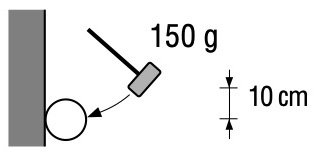
\includegraphics[scale=1]{K1.png}		& \SI{0,15}{\joule}	& 										& 								\\
02 				& 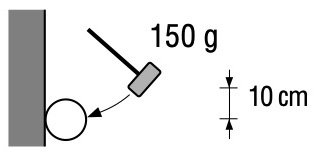
\includegraphics[scale=1]{K1.png}		& \SI{0,20}{\joule}	& 	AG1								& 1							\\
03 				& 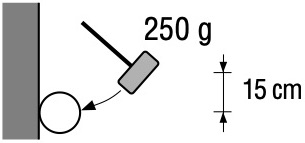
\includegraphics[scale=1]{K3.png}		& \SI{0,35}{\joule}	& 										& 								\\
04 				& 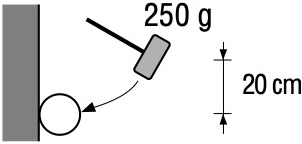
\includegraphics[scale=1]{K4.png}		& \SI{0,50}{\joule}	& 										& 3							\\
05 				& 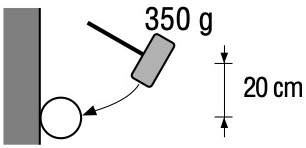
\includegraphics[scale=1]{K5.png}		& \SI{0,70}{\joule}	& 										& 								\\
06 				& 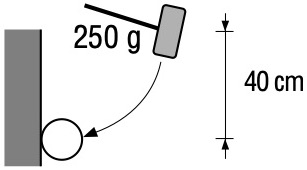
\includegraphics[scale=1]{K6.png}		& \SI{1}{\joule}		& 										& 								\\
07 				& 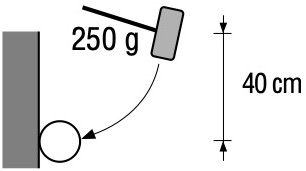
\includegraphics[scale=1]{K7.png}		& \SI{2}{\joule}		& 	AG2								& 5							\\
08 				& 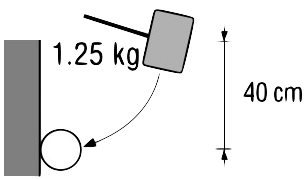
\includegraphics[scale=1]{K8.png}		& \SI{5}{\joule}		& 	AG3								& 								\\
08 				& 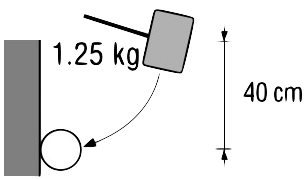
\includegraphics[scale=1]{K8.png}		& \SI{5}{\joule}		& 	AG3								& 								\\
09 				& 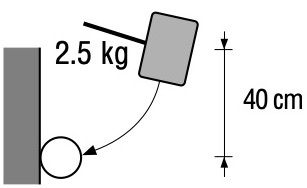
\includegraphics[scale=1]{K9.png}		& \SI{10}{\joule}		& 	AG3								& 								\\
10 				& 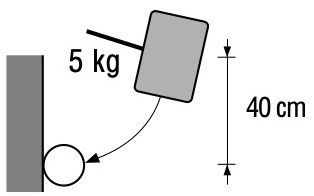
\includegraphics[scale=1]{K10.png}	& \SI{20}{\joule}		& 	AG4								& 								\\
\bottomrule
\end{tabularx}
\begin{tablenotes}
    \item[1] Corresponsdances avec le code AG de la classification des influences externes issu de la norme NF C 15-100.
\end{tablenotes}
\end{threeparttable} %note dans tableau
\end{table}
\end{minipage}
\hfill
\begin{minipage}[t]{0.39\linewidth}
\begin{table}[H]
\caption{Lettre additionnelle sur les informations supplémentaires spécifiques}
\begin{tabularx}{\linewidth}{P{1.5cm} X}
\toprule
\thead{Lettre}		& \thead{Signification} \\
\midrule
f							& Résistant aux huiles \\
\addlinespace
H							& Appareil à haute tension \\
\addlinespace
M							& Appareil en déplacement durant le test à l'eau \\
\addlinespace
S							& Appareil immobile durant le test à l'eau \\
\addlinespace
W							& Conditions environnementales spécifiées \\
\bottomrule
\end{tabularx}
\end{table}
\end{minipage}

%--------------------------------------
%ELECTROTECHNIQUE - SCHEMA DE LIAISON A LA TERRE
%--------------------------------------

%utiliser les environnement \begin{comment} \end{comment} pour mettre en commentaire le préambule une fois la programmation appelée dans le document maître (!ne pas oublier de mettre en commentaire \end{document}!)

\begin{comment}

\documentclass[a4paper, 11pt, twoside, fleqn]{memoir}

\usepackage{AOCDTF}

%--------------------------------------
%CANEVAS
%--------------------------------------

\newcommand\BoxColor{\ifcase\thechapshift blue!30\or brown!30\or pink!30\or cyan!30\or green!30\or teal!30\or purple!30\or red!30\or olive!30\or orange!30\or lime!30\or gray!\or magenta!30\else yellow!30\fi} %définition de la couleur des marqueurs de chapitre

\newcounter{chapshift} %compteur de chapitre du marqueur de chapitre
\addtocounter{chapshift}{-1}
	
\newif\ifFrame %instruction conditionnelle pour les couleurs des pages
\Frametrue

\pagestyle{plain}

% the main command; the mandatory argument sets the color of the vertical box
\newcommand\ChapFrame{%
\AddEverypageHook{%
\ifFrame
\ifthenelse{\isodd{\value{page}}}
  {\backgroundsetup{contents={%
  \begin{tikzpicture}[overlay,remember picture]
  \node[
  	rounded corners=3pt,
    fill=\BoxColor,
    inner sep=0pt,
    rectangle,
    text width=1.3cm,
    text height=5.5cm,
    align=center,
    anchor=north west
  ] 
  at ($ (current page.north west) + (-0cm,-2*\thechapshift cm) $) %nombre négatif = espacement des marqueurs entre les différents chapitres (à régler en fin de rédaction) (4.5cm vaut un espacement équivalement à la hauteur du marqueur, une page peut en contenir 6 avec cet espacement-la mais il est le plus équilibré)
    {\rotatebox{90}{\hspace*{.3cm}%
      \parbox[c][0.9cm][t]{5cm}{%
        \raggedright\textcolor{black}{\sffamily\textbf{\leftmark}}}}};
  \end{tikzpicture}}}
  }
  {\backgroundsetup{contents={%
  \begin{tikzpicture}[overlay,remember picture]
  \node[
  	rounded corners=3pt,
    fill=\BoxColor,
    inner sep=0pt,
    rectangle,
    text width=1.3cm,
    text height=5.5cm,
    align=center,
    anchor=north east
  ] 
  at ($ (current page.north east) + (-0cm,-2*\thechapshift cm) $) %nombre négatif = espacement des marqueurs entre les différents chapitres (à régler en fin de rédaction) (4.5cm vaut un espacement équivalement à la hauteur du marqueur, une page peut en contenir 6 avec cet espacement-la mais il est le plus équilibré)
    {\rotatebox{90}{\hspace*{.3cm}%
      \parbox[c][0.9cm][t]{5cm}{%
        \raggedright\textcolor{black}{\sffamily\textbf{\leftmark}}}}};
  \end{tikzpicture}}}%
  }
  \BgMaterial%
  \fi%
}%
  \stepcounter{chapshift}
}

\renewcommand\chaptermark[1]{\markboth{\thechapter.~#1}{}} %redéfinition du marqueur de chapitre pour ne contenir que le titre du chapitre %à personnaliser selon le nombre de chapitre dans le cours

%--------------------------------------
%corps du document
%--------------------------------------

\begin{document} %corps du document
	\openleft %début de chapitre à gauche

\end{comment}

\begin{landscape}
\begin{xltabular}{\linewidth}{p{0.3cm} m{2cm} X p{0.3cm} m{2cm} X p{0.3cm} m{2.2cm} X}
\caption{Descriptif des indices de protection} 
\\
\toprule
\multicolumn{3}{c}{\thead{Protection contre les corps solides}}	& \multicolumn{3}{c}{\thead{Lettre additionnelle\\Contact direct avec les parties dangereuses}}	& \multicolumn{3}{c}{\thead{Protection contre les liquides}} \\
\midrule
\endfirsthead %en-tête de la première page du tableau  

\toprule
\multicolumn{3}{c}{\thead{Protection contre les corps solides}}	& \multicolumn{3}{c}{\thead{Lettre additionnelle\\sur le contact direct avec les parties dangereuses}}	& \multicolumn{3}{c}{\thead{Protection contre les liquides}} \\
\midrule
\endhead %en-tête de la première page du tableau  

\addlinespace
\midrule %filet de milieu de tableau
\multicolumn{9}{r}{\small\textit{Page suivante}}
\endfoot %pied de page de toutes les pages du tableau

\bottomrule
\endlastfoot %pied de page de la dernièredu tableau

0 		& 									& Aucune protection	&	&	&	& 0 	&	&	Aucune protection \\
1 		& 	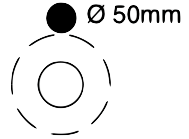
\includegraphics[scale=1.1]{1X.png} & Protégé contre les corps solides $\diameter \geq \SI{50}{\milli\meter}$  	&	A & 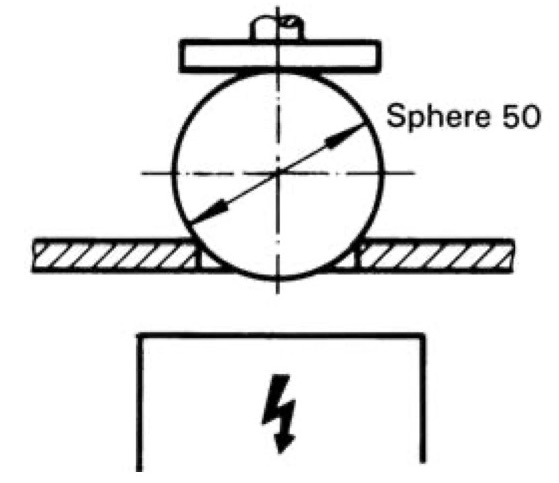
\includegraphics[width=2cm]{A.png}	&	Le dos de la main reste éloigné des parties dangereuses.	& 1 & 	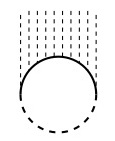
\includegraphics[scale=1.1]{X1.png}	&	Protégé contre les chutes verticales de gouttes d'eau (condensation) \\
2 		& 	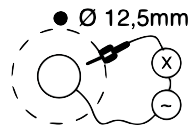
\includegraphics[scale=1.1]{2X.png} & Protégé contre les corps solides $\diameter \geq \SI{12,5}{\milli\meter}$  	& B	& 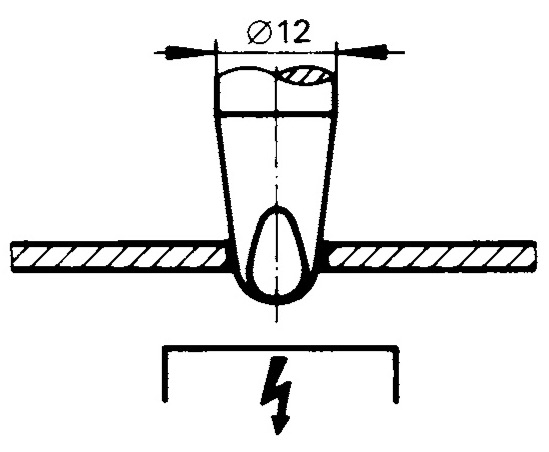
\includegraphics[width=2cm]{B.png}	&	L'introduction d'un doigt ne permet pas de toucher les parties dangereuses. & 2 & 	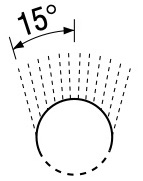
\includegraphics[scale=1.1]{X2.png}	&	Protégé contre les chutes de gouttes d'eau jusqu'à 15° de la verticale \\
3 		& 	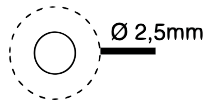
\includegraphics[scale=1.1]{3X.png} & Protégé contre les corps solides $\diameter \geq \SI{2,5}{\milli\meter}$  	& C	& 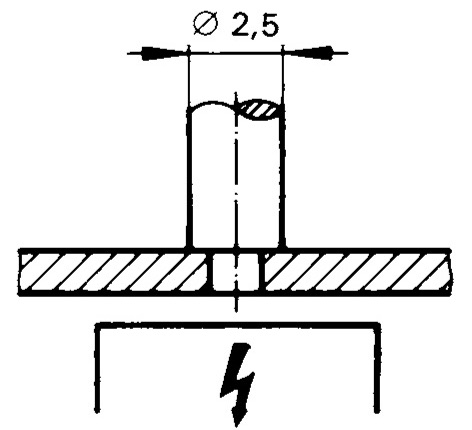
\includegraphics[width=2cm]{C.png}	&	L'introduction d'un outil ne permet pas de toucher les parties dangereuses. & 3 & 	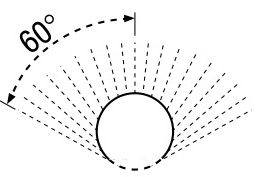
\includegraphics[scale=1.1]{X3.png}	&	Protégé contre l'eau de pluie jusqu'à 60° de la verticale \\
4 		& 	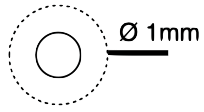
\includegraphics[scale=1.1]{4X.png} & Protégé contre les corps solides $\diameter \geq \SI{1}{\milli\meter}$  	& D	& 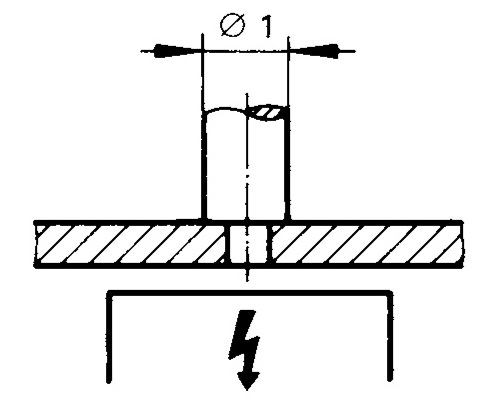
\includegraphics[width=2cm]{D.png}	&	L'introduction d'un outil fin ne permet pas de toucher les parties dangereuses. & 4 & 	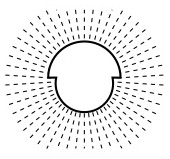
\includegraphics[scale=1.1]{X4.png}	&	Protégé contre les projections d'eau dans toutes les directions \\
5 		& 	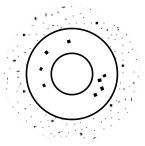
\includegraphics[scale=1.1]{5X.png} & Protégé contre la poussière (pas de dépot nuisible)  	& 	& & & 5 & 	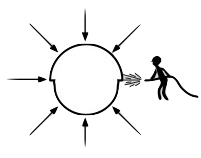
\includegraphics[scale=1.1]{X5.png}	&	Protégé contre les jets d'eau dans toutes les directions à la lance \\
6 		& 	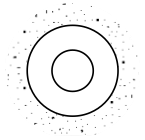
\includegraphics[scale=1.1]{6X.png} & Totalement protégé contre la poussière 	& 	& & & 6 & 	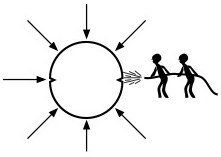
\includegraphics[scale=1.1]{X6.png}	&	Protégé contre les projections d'eau assimilables aux paquets de mer \\
 		&  & 	& 	& & & 7 & 	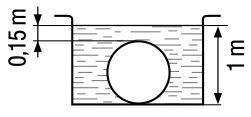
\includegraphics[scale=1.1]{X7.png}	&	Protégé contre les effets d'une immersion temporaire dans l'eau \\
		&  & 	& 	& & & 8 & 	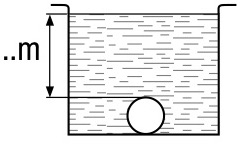
\includegraphics[scale=1.1]{X8.png}	&	Protégé contre les effets d'une immersion prolongée dans l'eau dans des conditions spécifiées \\
		&  & 	& 	& & & 9\tnote{1} & 	&	Protégé contre les jets d'eau haute pression et haute température mais pas nécessairement submersible \\
\end{xltabular}	

\end{landscape}

%\end{document}



\subsubsection{Classification des locaux selon l'IP}

Selon les locaux à équiper, leurs emplacements et les conditions particulières d'installation, la norme NF C 15-100 indique une protection minimale spécifiée par les indices IP et IK.

%--------------------------------------
%ELECTROTECHNIQUE - SCHEMA DE LIAISON A LA TERRE
%--------------------------------------

%utiliser les environnement \begin{comment} \end{comment} pour mettre en commentaire le préambule une fois la programmation appelée dans le document maître (!ne pas oublier de mettre en commentaire \end{document}!)

\begin{comment}

\documentclass[a4paper, 11pt, twoside, fleqn]{memoir}

\usepackage{AOCDTF}

%--------------------------------------
%CANEVAS
%--------------------------------------

\newcommand\BoxColor{\ifcase\thechapshift blue!30\or brown!30\or pink!30\or cyan!30\or green!30\or teal!30\or purple!30\or red!30\or olive!30\or orange!30\or lime!30\or gray!\or magenta!30\else yellow!30\fi} %définition de la couleur des marqueurs de chapitre

\newcounter{chapshift} %compteur de chapitre du marqueur de chapitre
\addtocounter{chapshift}{-1}
	
\newif\ifFrame %instruction conditionnelle pour les couleurs des pages
\Frametrue

\pagestyle{plain}

% the main command; the mandatory argument sets the color of the vertical box
\newcommand\ChapFrame{%
\AddEverypageHook{%
\ifFrame
\ifthenelse{\isodd{\value{page}}}
  {\backgroundsetup{contents={%
  \begin{tikzpicture}[overlay,remember picture]
  \node[
  	rounded corners=3pt,
    fill=\BoxColor,
    inner sep=0pt,
    rectangle,
    text width=1.3cm,
    text height=5.5cm,
    align=center,
    anchor=north west
  ] 
  at ($ (current page.north west) + (-0cm,-2*\thechapshift cm) $) %nombre négatif = espacement des marqueurs entre les différents chapitres (à régler en fin de rédaction) (4.5cm vaut un espacement équivalement à la hauteur du marqueur, une page peut en contenir 6 avec cet espacement-la mais il est le plus équilibré)
    {\rotatebox{90}{\hspace*{.3cm}%
      \parbox[c][0.9cm][t]{5cm}{%
        \raggedright\textcolor{black}{\sffamily\textbf{\leftmark}}}}};
  \end{tikzpicture}}}
  }
  {\backgroundsetup{contents={%
  \begin{tikzpicture}[overlay,remember picture]
  \node[
  	rounded corners=3pt,
    fill=\BoxColor,
    inner sep=0pt,
    rectangle,
    text width=1.3cm,
    text height=5.5cm,
    align=center,
    anchor=north east
  ] 
  at ($ (current page.north east) + (-0cm,-2*\thechapshift cm) $) %nombre négatif = espacement des marqueurs entre les différents chapitres (à régler en fin de rédaction) (4.5cm vaut un espacement équivalement à la hauteur du marqueur, une page peut en contenir 6 avec cet espacement-la mais il est le plus équilibré)
    {\rotatebox{90}{\hspace*{.3cm}%
      \parbox[c][0.9cm][t]{5cm}{%
        \raggedright\textcolor{black}{\sffamily\textbf{\leftmark}}}}};
  \end{tikzpicture}}}%
  }
  \BgMaterial%
  \fi%
}%
  \stepcounter{chapshift}
}

\renewcommand\chaptermark[1]{\markboth{\thechapter.~#1}{}} %redéfinition du marqueur de chapitre pour ne contenir que le titre du chapitre %à personnaliser selon le nombre de chapitre dans le cours

%--------------------------------------
%corps du document
%--------------------------------------

\begin{document} %corps du document
	\openleft %début de chapitre à gauche

\end{comment}

\captionof{table}{Classification des locaux}
\vspace{-1em}
\begin{minipage}[t]{0.49\linewidth}
\begin{tabularx}{\textwidth}[t]{c X c c}
\toprule
\multicolumn{2}{c}{\thead{Type de\\local}}																				& \thead{IP}	& \thead{IK}  \\
\midrule
\multicolumn{4}{p{0.95\textwidth}}{Locaux (ou emplacements) domestiques et analogues} \\
\middashrule \\
\multicolumn{2}{p{4.8cm}}{Auvents}																							& 24				& 07 \\
\multicolumn{2}{p{4.8cm}}{Bains (salle de)}																				& \multicolumn{2}{p{2.2cm}}{(voir salles d'eau)} \\
\multicolumn{2}{p{4.8cm}}{Bicyclettes, cyclomoteurs, voitures pour enfants (locaux pour)}			& 20				& 07 \\
\multicolumn{2}{p{4.8cm}}{Branchement eau, égout, chauffage}												& 23				& 02 \\
\multicolumn{2}{p{4.8cm}}{Buanderies}																					& 23				& 02 \\
\multicolumn{2}{p{4.8cm}}{Caves, celliers, garage, local avec chaudière}									& 20				& 02--07 \\
\multicolumn{2}{p{4.8cm}}{Chambres	}																					& 20				& 02 \\
\multicolumn{2}{p{4.8cm}}{Collecte des ordures (locaux pour)}												& 25				& 07 \\
\multicolumn{2}{p{4.8cm}}{Couloirs de cave}																			& 20				& 07 \\
\multicolumn{2}{p{4.8cm}}{Cours}																							& 24--25			& 02--07 \\
\multicolumn{2}{p{4.8cm}}{Cuisines}																						& 20				& 02 \\
\multicolumn{2}{p{4.8cm}}{Douches}																						& \multicolumn{2}{p{2.2cm}}{(voir salles d'eau)} \\
\multicolumn{2}{p{4.8cm}}{Escaliers intérieurs, coursives intérieures}										& 20				& 02--07 \\
\multicolumn{2}{p{4.8cm}}{Escaliers extérieures, coursives extérieures non couvertes}				& 24				& 07 \\
\multicolumn{2}{p{4.8cm}}{Coursives extérieures couvertes}														& 21				& 02 \\
\multicolumn{2}{p{4.8cm}}{Greniers (combles)}																			& 20				& 02 \\
\multicolumn{2}{p{4.8cm}}{Abris de jardins	}																			& 24--25			& 02--07 \\
\multicolumn{2}{p{4.8cm}}{Lieux d'aisances}																			& 20				& 02 \\
\multicolumn{2}{p{4.8cm}}{Locaux à poubelles}																		& 25				& 02--07 \\
\multicolumn{2}{p{4.8cm}}{Lingeries, salles de repassage}														& 21				& 02 \\
\multicolumn{2}{p{4.8cm}}{Rampes d'accès au garage}																& 25				& 07 \\
\multicolumn{2}{p{4.8cm}}{Salles d'eau, locaux contenant une baignoire ou une douche :	}		& 					& \\
& volume 0																& 27				& 02 \\
& volume 1																& 24				& 02 \\
& volume 2																& 23				& 02 \\
& volume 3																& 21				& 02 \\
\multicolumn{2}{p{4.8cm}}{Salles de séjour}																				& 20				& 02 \\
\multicolumn{2}{p{4.8cm}}{Séchoirs}																						& 21				& 02 \\
\end{tabularx}
\end{minipage}
\hfill
\begin{minipage}[t]{0.49\linewidth}
\begin{tabularx}{\textwidth}[t]{c X c c}
\toprule
\multicolumn{2}{c}{\thead{Type de\\local}}																				& \thead{IP}	& \thead{IK}  \\
\midrule
\multicolumn{4}{p{0.95\textwidth}}{Locaux (ou emplacements) domestiques et analogues} \\
\middashrule \\
\multicolumn{2}{p{4.8cm}}{Sous-sols}																						& 21				& 02/07 \\
\multicolumn{2}{p{4.8cm}}{Terrasses couvertes}																		& 21				& 02 \\
\multicolumn{2}{p{4.8cm}}{Toilettes (cabinets de)}																	& 21				& 02 \\
\multicolumn{2}{p{4.8cm}}{Vérandas}																						& 21				& 02 \\
\multicolumn{2}{p{4.8cm}}{Vides sanitaires}																				& 23				& 02--07 \\
\addlinespace
\midrule
\multicolumn{4}{p{0.95\textwidth}}{Locaux techniques} \\
\middashrule \\
\multicolumn{2}{p{4.8cm}}{Accumulateurs (salles d')}																& 23				& 02--07 \\
\multicolumn{2}{p{4.8cm}}{Ascenseurs (locaux des machines et locaux des poulies)}					& 20				& 07--08 \\	
\multicolumn{2}{p{4.8cm}}{Service électrique}																			& 20				& 07 \\
\multicolumn{2}{p{4.8cm}}{Salles des commandes}																	& 20				& 02 \\
\multicolumn{2}{p{4.8cm}}{Ateliers}																							& 21--23			& 07--08 \\
\multicolumn{2}{p{4.8cm}}{Laboratoires}																					& 21--23			& 02--07 \\
\multicolumn{2}{p{4.8cm}}{Laveurs de conditionnement d'air	}													& 24				& 07 \\
\multicolumn{2}{p{4.8cm}}{Garages (servant exclusivement au stationnement des véhicules) d'une surface n'excédant pas \SI{100}{\square\meter}}	& 21				& 07 \\
\multicolumn{2}{p{4.8cm}}{Laveurs de conditionnement d'air}													& 24				& 07 \\
\multicolumn{2}{p{4.8cm}}{Machines (salles de)}																		& 31				& 07--08 \\
\multicolumn{2}{p{4.8cm}}{Surpresseurs d'eau}																		& 23				& 07--08 \\
\multicolumn{2}{p{4.8cm}}{Chaufferies et locaux annexes :}														& 					& \\
&	 à charbon																																& 51--61			& 07--08 \\
&	 autres combustibles																												& 21				& 07--08 \\
&	 électriques																															& 21				& 07--08 \\
\addlinespace
\midrule
\multicolumn{4}{p{0.95\textwidth}}{Garages et parcs de stationnement couverts d'une surface supérieure à \SI{100}{\square\meter}} \\
\middashrule \\
\multicolumn{2}{p{4.8cm}}{Aires de stationnement}																	& 21				& 07--20 \\
\multicolumn{2}{p{4.8cm}}{Zones de lavage (à l'intérieur du local)}											& 25				& 07 \\
\multicolumn{2}{p{4.8cm}}{Zones de sécurité :}																		& 					&  \\
	&	à l'intérieur																														& 21				& 07 \\
	&	à l'extérieur																														& 24				& 07 \\
\multicolumn{2}{p{4.8cm}}{Zones de graissage}																			& 23				& 08 \\

\end{tabularx}
\end{minipage}
\begin{minipage}{0.49\textwidth}
\begin{tabularx}{\textwidth}{R}
\midrule
\small\textit{Colonne suivante} \\
\end{tabularx}
\end{minipage}
\hfill
\begin{minipage}{0.49\textwidth}
\begin{tabularx}{\textwidth}{R}
\midrule
\small\textit{Page suivante} \\
\end{tabularx}
\end{minipage}
\begin{minipage}[t]{0.49\linewidth}
\begin{tabularx}{\textwidth}[t]{c X c c}
\multicolumn{4}{l}{\small\textit{Page précédente}} \\
\midrule
\multicolumn{2}{c}{\thead{Type de\\local}}																				& \thead{IP}	& \thead{IK}  \\
\midrule
\multicolumn{4}{p{0.95\textwidth}}{Garages et parcs de stationnement couverts d'une surface supérieure à \SI{100}{\square\meter}} \\
\middashrule \\
\multicolumn{2}{p{4.8cm}}{Locaux de recharge de batteries}															& 23				& 07 \\
\multicolumn{2}{p{4.8cm}}{Ateliers}																								& 21				& 08 \\
\addlinespace
\midrule
\multicolumn{4}{p{0.95\textwidth}}{Locaux sanitaires à usage collectif} \\
\middashrule \\
\multicolumn{2}{p{4.8cm}}{Salles de lavabos individuels}																& 21				& 07 \\
\multicolumn{2}{p{4.8cm}}{Salles de WC à cuvettes (à l'anglaise)}													& 21				& 07 \\
\multicolumn{2}{p{4.8cm}}{Salles d'urinoirs}																					& 21				& 07 \\
\multicolumn{2}{p{4.8cm}}{Salles de lavabos collectifs}																	& 23				& 07 \\
\multicolumn{2}{p{4.8cm}}{Salles de WC à la turques, de douches à cabines individuelles, de douches collectives}								& 23				& 07 \\
\multicolumn{2}{p{4.8cm}}{Buanderies collectives}																		& 24				& 07 \\
\addlinespace
\midrule
\multicolumn{4}{p{0.95\textwidth}}{Bâtiments à usage collectif (autre que ERP)} \\
\middashrule \\
\multicolumn{2}{p{4.8cm}}{Bureaux}																							& 20				& 02 \\
\multicolumn{2}{p{4.8cm}}{Bibliothèques}																					& 20				& 02 \\
\multicolumn{2}{p{4.8cm}}{Salles d'archives}																				& 20				& 02 \\
\multicolumn{2}{p{4.8cm}}{Salles d'informatiques}																		& 20				& 02 \\
\multicolumn{2}{p{4.8cm}}{Salles de dessin}																					& 20				& 02 \\
\multicolumn{2}{p{4.8cm}}{Locaux regroupant les machines de reproduction de plans et de documents}			& 20				& 02 \\
\multicolumn{2}{p{4.8cm}}{Salles de tri}																						& 20				& 07 \\
\multicolumn{2}{p{4.8cm}}{Salles de restaurant et de cantine, grandes cuisines}							& 21				& 07 \\
\multicolumn{2}{p{4.8cm}}{Salles de sports}																					& 21				& 07--08 \\
\multicolumn{2}{p{4.8cm}}{Locaux de casernement}																		& 21				& 07 \\
\multicolumn{2}{p{4.8cm}}{Salles de réunion}																				& 20				& 02 \\
\multicolumn{2}{p{4.8cm}}{Salles d'attentes, salons, hall}																& 20				& 02 \\
\multicolumn{2}{p{4.8cm}}{Salles de consultation à usage médical, ne comportant pas d'équipements spécifiques}		& 20				& 02 \\
\multicolumn{2}{p{4.8cm}}{Salles de démonstration et d'exposition}												& 20				& 02 \\
\addlinespace
\midrule
\multicolumn{4}{p{0.95\textwidth}}{Locaux (ou emplacements) dans les exploitations agricoles} \\
\middashrule \\
\multicolumn{2}{p{4.8cm}}{Alcools (entrepôts de)}																		& 23				& 07 \\
\end{tabularx}
\end{minipage}
\hfill
\begin{minipage}[t]{0.49\linewidth}
\begin{tabularx}{\textwidth}[t]{c X c c}
\multicolumn{4}{l}{\small\textit{Colonne précédente}} \\
\midrule
\multicolumn{2}{c}{\thead{Type de\\local}}																				& \thead{IP}	& \thead{IK}  \\
\midrule
\multicolumn{4}{p{0.95\textwidth}}{Locaux (ou emplacements) dans les exploitations agricoles} \\
\middashrule \\
\multicolumn{2}{p{4.8cm}}{Bergeries fermées}																				& 35				& 07 \\
\multicolumn{2}{p{4.8cm}}{Buanderies}																					& 24				& 07 \\
\multicolumn{2}{p{4.8cm}}{Battages de céréales}																		& 50				& 07 \\
\multicolumn{2}{p{4.8cm}}{Bûchers}																							& 30				& 10 \\
\multicolumn{2}{p{4.8cm}}{Caves de distillation}																		& 23				& 07 \\
\multicolumn{2}{p{4.8cm}}{Chais (vin)	}																					& 23				& 07 \\
\multicolumn{2}{p{4.8cm}}{Cours}																							& 35				& 07 \\
\multicolumn{2}{p{4.8cm}}{\'Elevages de volailles}																	& 35				& 07 \\
\multicolumn{2}{p{4.8cm}}{\'Ecuries}																						& 35				& 07 \\
\multicolumn{2}{p{4.8cm}}{Engrais (dépôts d')}																			& 50				& 07 \\
\multicolumn{2}{p{4.8cm}}{\'Etables}																						& 35				& 07 \\
\multicolumn{2}{p{4.8cm}}{Fumières}																						& 24				& 07 \\
\multicolumn{2}{p{4.8cm}}{Fenils}																							& 50				& 07 \\
\multicolumn{2}{p{4.8cm}}{Fourrage (entrepôts de)}																	& 50				& 07 \\
\multicolumn{2}{p{4.8cm}}{Greniers, granges}																			& 50				& 07 \\
\multicolumn{2}{p{4.8cm}}{Paille (entrepôts de)}																		& 50				& 07 \\
\multicolumn{2}{p{4.8cm}}{Serres}																							& 23				& 07 \\
\multicolumn{2}{p{4.8cm}}{Silos à céréales}																				& 50				& 07 \\
\multicolumn{2}{p{4.8cm}}{Traies (salle de)}																				& 35				& 07 \\
\multicolumn{2}{p{4.8cm}}{Porcheries}																						& 35				& 07 \\
\multicolumn{2}{p{4.8cm}}{Poulaillers}																						& 35				& 07 \\
\addlinespace
\midrule
\multicolumn{4}{p{0.95\textwidth}}{Installations diverses} \\
\middashrule \\
\multicolumn{2}{p{4.8cm}}{Terrains de camping et caravaning}													& 34				& 07 \\
\multicolumn{2}{p{4.8cm}}{Quais de ports de plaisance}															& 34				& 08 \\
\multicolumn{2}{p{4.8cm}}{Chantiers}																						& 44				& 08 \\
\multicolumn{2}{p{4.8cm}}{Quais de chargement}																		& 35				& 08 \\
\multicolumn{2}{p{4.8cm}}{Rues, cours, jardins et autres emplacements extérieurs}					& 34--35			& 07 \\
\multicolumn{2}{p{4.8cm}}{\'Etablissement forains}																	& 33				& 08 \\
\multicolumn{2}{p{4.8cm}}{Piscines :}																						& 					&	  \\
& volume 0																																& 28				& 02 \\
& volume 1																																& 25				& 02 \\
& volume 2																																& 22--24			& 02 \\
\multicolumn{2}{p{4.8cm}}{Saunas}																							& 34				& 02 \\
\multicolumn{2}{p{4.8cm}}{Bassins de fontaines}																		& 37				& 02 \\
\multicolumn{2}{p{4.8cm}}{Traitements des eaux (local de)}														& 24--25			& 07--08 \\
\addlinespace
\midrule
\multicolumn{4}{p{0.95\textwidth}}{Installations thermodynamiques, chambres climatisées et chambres froides} \\
\middashrule \\
\end{tabularx}
\end{minipage}
\begin{minipage}[b]{0.49\textwidth}
\begin{xltabular}{\textwidth}{R}
\midrule
\small\textit{Colonne suivante} \\
\end{xltabular}
\end{minipage}
\hfill
\begin{minipage}[b]{0.49\textwidth}
\begin{xltabular}{\textwidth}{R}
\midrule
\small\textit{Page suivante} \\
\end{xltabular}
\end{minipage}
\begin{minipage}[t]{0.49\linewidth}
\begin{tabularx}{\textwidth}[t]{c X c c}
\multicolumn{4}{l}{\small\textit{Page précédente}} \\
\midrule
\multicolumn{2}{c}{\thead{Type de\\local}}																				& \thead{IP}	& \thead{IK}  \\
\midrule
\multicolumn{4}{p{0.95\textwidth}}{Installations thermodynamiques, chambres climatisées et chambres froides} \\
\middashrule \\
\multicolumn{2}{p{4.8cm}}{Température < \SI{-10}{\celsius}}												&	23				&	07 \\	
\multicolumn{2}{p{4.8cm}}{Hauteur au dessus du sol :}															& 					&  \\
& \SIrange[range-phrase=\ à\ ]{0}{1,10}{\meter}																		& 24				& 07 \\
& \SIrange[range-phrase=\ à\ ]{1,10}{2}{\meter}																		& 21				& 07 \\
& au-dessus de \SI{2}{\meter}																									& 21				& 07 \\
& sous l'évaporateur ou tube																									& 21				& 07 \\
& écoulement d'eau																													& 21				& 07 \\
\multicolumn{2}{p{4.8cm}}{Plafond et jusqu'à \SI{10}{\centi\meter} en-dessous}	 				&	23				&	07 \\	
\multicolumn{2}{p{4.8cm}}{Compresseur :}																			& 					&  \\
& local																																		& 21				& 08 \\
& monobloc placé à l'extérieur ou en terrasse																				& 34				& 08 \\
\midrule
\multicolumn{4}{p{0.95\textwidth}}{\'Etablissements industriels} \\
\middashrule \\
\multicolumn{2}{p{4.8cm}}{Abattoirs}																	 				&	55				&	08 \\	
\multicolumn{2}{p{4.8cm}}{Accumulateurs (fabrication d')}										 				&	33				&	07 \\	
\multicolumn{2}{p{4.8cm}}{Acide (fabrication et dépôts)}										 				&	33				&	07 \\	
\multicolumn{2}{p{4.8cm}}{Alcool (fabrication et dépôts)}										 				&	33				&	07 \\	
\multicolumn{2}{p{4.8cm}}{Aluminium (fabrication et dépôts)}										 		&	51--53		&	08 \\	
\multicolumn{2}{p{4.8cm}}{Animaux (élevage et engraissement)}										 	&	45				&	07 \\	
\multicolumn{2}{p{4.8cm}}{Asphaltes, bitume (dépôts d')}										 				&	53				&	07 \\	
\multicolumn{2}{p{4.8cm}}{Battage et cardage des laines}											 				&	50				&	08 \\	
\multicolumn{2}{p{4.8cm}}{Blanchisseries}																 				&	23--24		&	07 \\	
\multicolumn{2}{p{4.8cm}}{Bois (travail du)}																 			&	50				&	08 \\
\multicolumn{2}{p{4.8cm}}{Boucheries}																		 			&	24--25		&	07 \\	
\multicolumn{2}{p{4.8cm}}{Boucheries}																		 			&	24--25		&	07 \\	
\multicolumn{2}{p{4.8cm}}{Brasseries}																		 			&	24				&	07 \\	
\multicolumn{2}{p{4.8cm}}{Briqueteries}																		 		&	53--54		&	08 \\	
\multicolumn{2}{p{4.8cm}}{Caoutchouc (fabrication et transformation)}								 	&	54				&	07 \\	
\multicolumn{2}{p{4.8cm}}{Carbure (fabrication et dépôts)}								 					&	51				&	07 \\	
\multicolumn{2}{p{4.8cm}}{Cartoucherie}								 												&	53				&	08 \\	
\multicolumn{2}{p{4.8cm}}{Cartons (fabrication de}																&	33				&	07 \\	
\multicolumn{2}{p{4.8cm}}{Carrières}									 												&	55				&	08 \\
\multicolumn{2}{p{4.8cm}}{Celluloïd (fabrication d'objets}														&	30				&	08 \\	
\multicolumn{2}{p{4.8cm}}{Cellulose (fabrication)}									 								&	34				&	08 \\	
\end{tabularx}
\end{minipage}
\hfill
\begin{minipage}[t]{0.49\linewidth}
\begin{tabularx}{\textwidth}[t]{c X c c}
\multicolumn{4}{l}{\small\textit{Colonne précédente}} \\
\midrule
\multicolumn{2}{c}{\thead{Type de\\local}}																				& \thead{IP}	& \thead{IK}  \\
\midrule
\multicolumn{4}{p{0.95\textwidth}}{\'Etablissements industriels} \\
\middashrule \\
\multicolumn{2}{p{4.8cm}}{Charbon (entrepôts de)}									 							&	54				&	08 \\	
\multicolumn{2}{p{4.8cm}}{Charcuteries}									 											&	24				&	07 \\	
\multicolumn{2}{p{4.8cm}}{Chaudronneries}									 										&	30				&	08 \\	
\multicolumn{2}{p{4.8cm}}{Chaux (fours à)}									 										&	50				&	08 \\	
\multicolumn{2}{p{4.8cm}}{Chiffons (entrepôts de)}									 							&	30				&	07 \\	
\multicolumn{2}{p{4.8cm}}{Chlore (fabrication et dépôts)}									 					&	33				&	07 \\	
\multicolumn{2}{p{4.8cm}}{Chromage}									 												&	33				&	07 \\	
\multicolumn{2}{p{4.8cm}}{Cimenterie}									 												&	50				&	08 \\	
\multicolumn{2}{p{4.8cm}}{Cokerie}									 													&	53				&	08 \\	
\multicolumn{2}{p{4.8cm}}{Colle (fabrication de)}									 								&	33				&	07 \\
\multicolumn{2}{p{4.8cm}}{Chaines d'embouteillage}									 							&	35				&	08 \\	
\multicolumn{2}{p{4.8cm}}{Combustibles liquides (dépôts de)}												&	31--33		&	08 \\	
\multicolumn{2}{p{4.8cm}}{Corps gras (traitement de)}									 						&	51				&	07 \\	
\multicolumn{2}{p{4.8cm}}{Cuir (fabrication et dépôts de)}									 					&	31				&	08 \\	
\multicolumn{2}{p{4.8cm}}{Cuivre (traitement des minéraux)}									 				&	31				&	08 \\	
\multicolumn{2}{p{4.8cm}}{Décapage}									 												&	54				&	08 \\	
\multicolumn{2}{p{4.8cm}}{Détersifs (fabrication de produits)}									 			&	53				&	07 \\	
\multicolumn{2}{p{4.8cm}}{Distillerie}									 												&	33				&	07 \\	
\multicolumn{2}{p{4.8cm}}{\'Electrolyse}									 											&	03				&	08 \\	
\multicolumn{2}{p{4.8cm}}{Encre (fabrication d')}									 								&	31				&	07 \\	
\multicolumn{2}{p{4.8cm}}{Engrais (fabrication et dépôts de)}				 								&	53				&	07 \\	
\multicolumn{2}{p{4.8cm}}{Explosifs (fabrication et dépôts de)}				 								&	55				&	08 \\	
\multicolumn{2}{p{4.8cm}}{Fer (fabrication et traitement de)}				 									&	51				&	08 \\	
\multicolumn{2}{p{4.8cm}}{Filatures}									 													&	50			&	07 \\	
\multicolumn{2}{p{4.8cm}}{Fourrures (battage)}									 									&	50			&	07 \\	
\multicolumn{2}{p{4.8cm}}{Fromageries}									 											&	25			&	07 \\	
\multicolumn{2}{p{4.8cm}}{Gaz (usines et depôts de)}									 						&	31			&	08 \\	
\multicolumn{2}{p{4.8cm}}{Goudron (traitement de)}									 							&	33			&	07 \\	
\multicolumn{2}{p{4.8cm}}{Graineteries}									 											&	50			&	07 \\	
\multicolumn{2}{p{4.8cm}}{Gravures de métaux}																	&	33			&	07 \\	
\multicolumn{2}{p{4.8cm}}{Huile (extraction de)}																	&	31			&	07 \\	
\multicolumn{2}{p{4.8cm}}{Hydrocarbures (fabrication de)}														&	33--34	&	08 \\	
\multicolumn{2}{p{4.8cm}}{Imprimeries}																				&	20			&	08 \\	
\multicolumn{2}{p{4.8cm}}{Laiteries}																						&	25			&	07 \\	
\multicolumn{2}{p{4.8cm}}{Laveries, lavoirs publics}																&	25			&	07 \\	
\multicolumn{2}{p{4.8cm}}{Liqueurs (fabrication de)}																&	21			&	07 \\	
\end{tabularx}
\end{minipage}
\begin{minipage}[b]{0.49\textwidth}
\begin{xltabular}{\textwidth}{R}
\midrule
\small\textit{Colonne suivante} \\
\end{xltabular}
\end{minipage}
\hfill
\begin{minipage}[b]{0.49\textwidth}
\begin{xltabular}{\textwidth}{R}
\midrule
\small\textit{Page suivante} \\
\end{xltabular}
\end{minipage}
\begin{minipage}[t]{0.49\linewidth}
\begin{tabularx}{\textwidth}[t]{c X c c}
\multicolumn{4}{l}{\small\textit{Page précédente}} \\
\midrule
\multicolumn{2}{c}{\thead{Type de\\local}}																				& \thead{IP}	& \thead{IK}  \\
\midrule
\multicolumn{4}{p{0.95\textwidth}}{\'Etablissements industriels} \\
\middashrule \\
\multicolumn{2}{p{4.8cm}}{Liquides halogénés (emploi de)}													&	21			&	08 \\	
\multicolumn{2}{p{4.8cm}}{Liquides inflammables (dépôts, ateliers ou l'on emploie des)}			&	21			&	08 \\	
\multicolumn{2}{p{4.8cm}}{Magnésium (fabrication, travail et depôts de)}								&	31			&	07 \\	
\multicolumn{2}{p{4.8cm}}{Machines (salle des)}																	&	20			&	08 \\	
\multicolumn{2}{p{4.8cm}}{Matières plastiques (fabrication de)}												&	51			&	08 \\	
\multicolumn{2}{p{4.8cm}}{Menuiseries}																				&	50			&	08 \\	
\multicolumn{2}{p{4.8cm}}{Métaux (traitement de)}									 							&	31--33	&	08 \\	
\multicolumn{2}{p{4.8cm}}{Moteurs thermiques (essai de)}									 					&	30			&	08 \\	
\multicolumn{2}{p{4.8cm}}{Munitions (dépôts de)}									 								&	33			&	08 \\	
\multicolumn{2}{p{4.8cm}}{Nickel (traitement des minérais)}									 				&	33			&	08 \\	
\multicolumn{2}{p{4.8cm}}{Ordures ménagères (traitement d')}								 				&	53--54	&	07 \\	
\multicolumn{2}{p{4.8cm}}{Papiers (fabriques de)}													 				&	33--34	&	07 \\	
\multicolumn{2}{p{4.8cm}}{Papiers (dépôts de)}													 					&	31			&	07 \\	
\multicolumn{2}{p{4.8cm}}{Parfum (fabrication et dépôts de)}													&	31			&	07 \\	
\multicolumn{2}{p{4.8cm}}{Pâte à papiers (préparation de)}													&	34			&	07 \\	
\multicolumn{2}{p{4.8cm}}{Peinture (fabrication et dépôts de)}												&	33			&	08 \\	
\multicolumn{2}{p{4.8cm}}{Plâtre (broyage et dépôts de)}														&	50			&	07 \\	
\multicolumn{2}{p{4.8cm}}{Poudreries}																					&	55			&	07 \\	
\multicolumn{2}{p{4.8cm}}{Produits chimiques (fabrication de)}												&	30--50	&	08 \\	
\multicolumn{2}{p{4.8cm}}{Raffinerie de pétrole}																	&	34			&	07 \\	
\multicolumn{2}{p{4.8cm}}{Salaisons}																					&	33			&	07 \\	
\multicolumn{2}{p{4.8cm}}{Savons (fabrication de)}																&	31			&	07 \\	
\multicolumn{2}{p{4.8cm}}{Scieries}																						&	50			&	08 \\	
\multicolumn{2}{p{4.8cm}}{Serrureries}																					&	30			&	08 \\	
\multicolumn{2}{p{4.8cm}}{Silos à céréales ou à sucre}															&	50			&	07 \\	
\multicolumn{2}{p{4.8cm}}{Soies et crins (préparation de)}														&	50			&	08 \\	
\multicolumn{2}{p{4.8cm}}{Soude (fabrication et dépôts de)}													&	33			&	07 \\	
\multicolumn{2}{p{4.8cm}}{Soude (traitement de)}																		&	51			&	07 \\	
\multicolumn{2}{p{4.8cm}}{Spiritueux (entrepôts de)}																&	33			&	07 \\	
\multicolumn{2}{p{4.8cm}}{Sucreries}																					&	55			&	07 \\	
\multicolumn{2}{p{4.8cm}}{Tanneries}																					&	35			&	07 \\	
\end{tabularx}
\end{minipage}
\hfill
\begin{minipage}[t]{0.49\linewidth}
\begin{tabularx}{\textwidth}[t]{c X c c}
\multicolumn{4}{l}{\small\textit{Colonne précédente}} \\
\midrule
\multicolumn{2}{c}{\thead{Type de\\local}}																				& \thead{IP}	& \thead{IK}  \\
\midrule
\multicolumn{4}{p{0.95\textwidth}}{\'Etablissements industriels} \\
\middashrule \\
\multicolumn{2}{p{4.8cm}}{Teintureries}																				&	35			&	07 \\	
\multicolumn{2}{p{4.8cm}}{Textiles et tissus (fabrication de)}													&	51			&	08 \\	
\multicolumn{2}{p{4.8cm}}{Vernis (fabrication et application de)}											&	33			&	08 \\	
\multicolumn{2}{p{4.8cm}}{Verreries}																					&	33			&	08 \\	
\multicolumn{2}{p{4.8cm}}{Zinc (travail du)}																			&	31			&	08 \\	
\midrule
\multicolumn{4}{p{0.95\textwidth}}{\'Etablissements recevant du public (ERP)} \\
\middashrule \\
L 	& \multicolumn{3}{p{0.75\textwidth}}{Salles d'audition, de conférence, de réunion, de spectacles ou à usages multiples :} \\
& salles																																	& 20			& 02--07 \\
& cages de scènes																													& 20			& 08 \\
& magasin de décors																												& 20			& 08 \\
& locaux des perruquiers et des cordonniers																			& 20			& 07 \\
M 	& \multicolumn{3}{p{0.8\textwidth}}{Magasins de vente, centres commerciaux :} \\
& locaux de ventes																												& 20			& 08 \\
& stockages et manipulations de matériels d'emballages															& 20			& 08 \\
N	& Restaurants et débits de boissons																					& 20			& 02 \\
O	& Hôtels et pensions de familles																							& 20			& 02 \\
P	& Salles de danse et salles de jeux																						& 20			& 07 \\
R 	& \multicolumn{3}{p{0.75\textwidth}}{\'Etablissements d'enseignement, colonies de vacances :} \\
& salles	 d'enseignement																										& 20			& 02 \\
& dortoirs																																& 20			& 07 \\
S	&  Bibliothèques, centres de documentation																		& 20			& 02 \\
T 	& \multicolumn{3}{p{0.75\textwidth}}{Expositions :} \\
& halls et salles																														& 21			& 07 \\
& locaux de réceptions de matériels et de marchandises															& 20			& 08 \\
U 	& \multicolumn{3}{p{0.75\textwidth}}{\'Etablissements sanitaires :} \\
& chambres																															& 20			& 02 \\
& incinérations																														& 21			& 07--08 \\
& blocs opératoires																												& 20			& 07 \\
\end{tabularx}
\end{minipage}
\begin{minipage}[b]{0.49\textwidth}
\begin{xltabular}{\textwidth}{R}
\midrule
\small\textit{Colonne suivante} \\
\end{xltabular}
\end{minipage}
\hfill
\begin{minipage}[b]{0.49\textwidth}
\begin{xltabular}{\textwidth}{R}
\midrule
\small\textit{Page suivante} \\
\end{xltabular}
\end{minipage}
\begin{minipage}[t]{0.49\linewidth}
%\begin{threeparttable}
\begin{tabularx}{\textwidth}[t]{c X c c}
\multicolumn{4}{l}{\small\textit{Page précédente}} \\
\midrule
\multicolumn{2}{c}{\thead{Type de\\local}}																				& \thead{IP}	& \thead{IK}  \\
\midrule
\multicolumn{4}{p{0.95\textwidth}}{\'Etablissements recevant du public (ERP)} \\
\middashrule \\
U 	& \multicolumn{3}{p{0.75\textwidth}}{\'Etablissements sanitaires :} \\
& stérilisations centralisées																									& 24--25		& 02--07 \\
& pharmacies et laboratoires avec plus de \SI{10}{\liter} de liquides inflammatoires				& 21--23		& 02--07 \\
V & \'Etablissement de cultes 																									& 20				& 02 \\
W & Administrations et banques																								& 20				& 02 \\
X 	& \multicolumn{3}{p{0.75\textwidth}}{\'Etablissements sportifs couverts :} \\
& Salles																																	& 21				& 07--08 \\
& Locaux contenant des installations frigorifiques																	& 21				& 08 \\
Y & Musées																															& 20				& 02 \\
PA & \'Etablissement de plein air 																							& 25				& 08--10 \\
CT & Chapiteaux et tentes 																										& 44($^1$)	& 08 \\
SG & Structures gonflables 																									& 44				& 08 \\
PS & Parc de stationnement couvert																						& 21				& 07--10 \\
\midrule
\multicolumn{4}{p{0.95\textwidth}}{Locaux communs aux établissements recevant du public} \\
\middashrule \\
\multicolumn{2}{p{4.8cm}}{Dépôts, réserve}																		&	20			&	08 \\	
\multicolumn{2}{p{4.8cm}}{Locaux d'emballage}																&	20			&	08 \\	
\multicolumn{2}{p{4.8cm}}{Locaux d'archive et de stockage}												&	20			&	02 \\	
\multicolumn{2}{p{4.8cm}}{Films et supports magnétiques}												&	20			&	08 \\	
\multicolumn{2}{p{4.8cm}}{Lingeries}																				&	21			&	02 \\	
\multicolumn{2}{p{4.8cm}}{Blanchisseries}																			&	24			&	07 \\	
\multicolumn{2}{p{4.8cm}}{Ateliers divers}																			&	21			&	07--08 \\	
\multicolumn{2}{p{4.8cm}}{Cuisines (grandes)$^2$}													&				& \\
\midrule
\multicolumn{4}{p{0.95\textwidth}}{Locaux commerciaux, boutiques et annexes} \\
\middashrule \\
\multicolumn{2}{p{4.8cm}}{Armuries (réserves et ateliers d')}												&	31--33			&	08 \\	
\multicolumn{2}{p{4.8cm}}{Blanchisseries (laveries)}															&	24					&	07 \\
\end{tabularx}
%\end{threeparttable}
\end{minipage}
\hfill
\begin{minipage}[t]{0.49\linewidth}
\begin{tabularx}{\textwidth}[t]{c X c c}
\multicolumn{4}{l}{\small\textit{Colonne précédente}} \\
\midrule
\multicolumn{2}{c}{\thead{Type de\\local}}																				& \thead{IP}	& \thead{IK}  \\
\midrule
\multicolumn{4}{p{0.95\textwidth}}{Locaux commerciaux, boutiques et annexes} \\
\middashrule \\
\multicolumn{2}{p{4.8cm}}{Boucherie :}																				& 					&  \\
 & Boutique																															& 24				& 07 \\
 & Chambre froide																													& 23				& 07 \\
\multicolumn{2}{p{4.8cm}}{Boulangerie-pâtisserie (fournil)}												&	50				&	07 \\
\multicolumn{2}{p{4.8cm}}{Brûlerie cafés}																		&	21				&	02 \\
\multicolumn{2}{p{4.8cm}}{Charbon, bois, mazout}																&	20				&	08 \\
\multicolumn{2}{p{4.8cm}}{Charcuterie (fabrication de)}														&	24				&	07 \\
\multicolumn{2}{p{4.8cm}}{Confiserie (fabrication de)}														&	20				&	02 \\
\multicolumn{2}{p{4.8cm}}{Cordonnerie}																			&	20				&	02 \\
\multicolumn{2}{p{4.8cm}}{Crèmerie, fromagerie}															&	24				&	02 \\
\multicolumn{2}{p{4.8cm}}{Droguerie, peinture (réserve de)}											&	33				&	07 \\
\multicolumn{2}{p{4.8cm}}{\'Ebenisterie, menuiserie}														&	50				&	07 \\
\multicolumn{2}{p{4.8cm}}{Exposition, galerie d'art}														&	20				&	02--07 \\
\multicolumn{2}{p{4.8cm}}{Fleuriste}																				&	24				&	02 \\
\multicolumn{2}{p{4.8cm}}{Fourrure}																				&	20				&	02 \\
\multicolumn{2}{p{4.8cm}}{Fruits et légumes}																&	24				&	07 \\
\multicolumn{2}{p{4.8cm}}{Graineterie}																			&	50				&	07 \\
\multicolumn{2}{p{4.8cm}}{Libraire, papeterie}																&	20				&	02 \\
\multicolumn{2}{p{4.8cm}}{Mécanique, accessoires de motos et vélos}							&	20				&	08 \\
\multicolumn{2}{p{4.8cm}}{Messageries}																		&	20				&	08 \\
\multicolumn{2}{p{4.8cm}}{Meuble (antiquités et brocantes de)}										&	20				&	07 \\
\multicolumn{2}{p{4.8cm}}{Miroiterie (atelier de)}															&	20				&	07 \\
\multicolumn{2}{p{4.8cm}}{Papiers peints (réserve de)}													&	21				&	07 \\
\multicolumn{2}{p{4.8cm}}{Parfumerie (réserve de)}														&	31				&	02 \\
\multicolumn{2}{p{4.8cm}}{Pharmacie (réserve de)}														&	20				&	02 \\
\multicolumn{2}{p{4.8cm}}{Photographie (laboratoire de)}												&	23				&	02 \\
\multicolumn{2}{p{4.8cm}}{Plomberie et sanitaire (réserve de)}										&	20				&	07 \\
\multicolumn{2}{p{4.8cm}}{Poissonnerie}																		&	20				&	07 \\
\multicolumn{2}{p{4.8cm}}{Pressing et teinturerie}															&	23				&	02 \\
\multicolumn{2}{p{4.8cm}}{Quincaillerie}																		&	20				&	07 \\
\multicolumn{2}{p{4.8cm}}{Serrurerie}																			&	20				&	07--08 \\
\multicolumn{2}{p{4.8cm}}{Spiritueux, vins et alcools (caves de stockages de)}				&	23				&	07 \\
\multicolumn{2}{p{4.8cm}}{Tapissier (cardage de)}															&	50				&	07 \\
\multicolumn{2}{p{4.8cm}}{Tailleur, vêtement (réserve de)}											&	20				&	02 \\
\multicolumn{2}{p{4.8cm}}{Toilette animaux, clinique vétérinaire}									&	35				&	07 \\
\bottomrule
\end{tabularx}
\end{minipage}
\begin{minipage}[b]{0.49\textwidth}
\begin{threeparttable}
\begin{tabularx}{\textwidth}[b]{R}
\midrule
\small\textit{Colonne suivante} \\
\end{tabularx}
\begin{tablenotes}
    \item[1] IP24 - IK08 pour les luminaires\,;
    \item[2] Se reporter au guide spécialisé UTE C15-201.
\end{tablenotes}
\end{threeparttable}
\end{minipage}

%\end{document}



\subsection{Transformateur d'isolement\label{subsec:tranformateur_isolement}}

Le \emph{transformateur d'isolement} a pour but d'isoler l'utilisateur du réseau électrique. On le retrouve généralement dans les salles de bains d'ERP tels que les hôtels, intégré aux sèches-cheveux et rasoirs muraux.\\ 

%--------------------------------------
%ELECTROTECHNIQUE - SCHEMA DE LIAISON A LA TERRE
%--------------------------------------

%utiliser les environnement \begin{comment} \end{comment} pour mettre en commentaire le préambule une fois la programmation appelée dans le document maître (!ne pas oublier de mettre en commentaire \end{document}!)

\begin{comment}

\documentclass[a4paper, 11pt, twoside, fleqn]{memoir}

\usepackage{AOCDTF}

%--------------------------------------
%CANEVAS
%--------------------------------------

\newcommand\BoxColor{\ifcase\thechapshift blue!30\or brown!30\or pink!30\or cyan!30\or green!30\or teal!30\or purple!30\or red!30\or olive!30\or orange!30\or lime!30\or gray!\or magenta!30\else yellow!30\fi} %définition de la couleur des marqueurs de chapitre

\newcounter{chapshift} %compteur de chapitre du marqueur de chapitre
\addtocounter{chapshift}{-1}
	
\newif\ifFrame %instruction conditionnelle pour les couleurs des pages
\Frametrue

\pagestyle{plain}

% the main command; the mandatory argument sets the color of the vertical box
\newcommand\ChapFrame{%
\AddEverypageHook{%
\ifFrame
\ifthenelse{\isodd{\value{page}}}
  {\backgroundsetup{contents={%
  \begin{tikzpicture}[overlay,remember picture]
  \node[
  	rounded corners=3pt,
    fill=\BoxColor,
    inner sep=0pt,
    rectangle,
    text width=1.3cm,
    text height=5.5cm,
    align=center,
    anchor=north west
  ] 
  at ($ (current page.north west) + (-0cm,-2*\thechapshift cm) $) %nombre négatif = espacement des marqueurs entre les différents chapitres (à régler en fin de rédaction) (4.5cm vaut un espacement équivalement à la hauteur du marqueur, une page peut en contenir 6 avec cet espacement-la mais il est le plus équilibré)
    {\rotatebox{90}{\hspace*{.3cm}%
      \parbox[c][0.9cm][t]{5cm}{%
        \raggedright\textcolor{black}{\sffamily\textbf{\leftmark}}}}};
  \end{tikzpicture}}}
  }
  {\backgroundsetup{contents={%
  \begin{tikzpicture}[overlay,remember picture]
  \node[
  	rounded corners=3pt,
    fill=\BoxColor,
    inner sep=0pt,
    rectangle,
    text width=1.3cm,
    text height=5.5cm,
    align=center,
    anchor=north east
  ] 
  at ($ (current page.north east) + (-0cm,-2*\thechapshift cm) $) %nombre négatif = espacement des marqueurs entre les différents chapitres (à régler en fin de rédaction) (4.5cm vaut un espacement équivalement à la hauteur du marqueur, une page peut en contenir 6 avec cet espacement-la mais il est le plus équilibré)
    {\rotatebox{90}{\hspace*{.3cm}%
      \parbox[c][0.9cm][t]{5cm}{%
        \raggedright\textcolor{black}{\sffamily\textbf{\leftmark}}}}};
  \end{tikzpicture}}}%
  }
  \BgMaterial%
  \fi%
}%
  \stepcounter{chapshift}
}

\renewcommand\chaptermark[1]{\markboth{\thechapter.~#1}{}} %redéfinition du marqueur de chapitre pour ne contenir que le titre du chapitre %à personnaliser selon le nombre de chapitre dans le cours

%--------------------------------------
%corps du document
%--------------------------------------

\begin{document} %corps du document
	\openleft %début de chapitre à gauche

\end{comment}

\begin{wrapfigure}{R}{0pt} %insertion figure dans texte
\begin{circuitikz}[circuit ee IEC]
%\DrawGrid{(-1,-5)}{(7,3)} %grille d'aide pour le placement des objets

\fill [gray!50] (-1,-3.5) -- (5,-3.5) -- (5,-3.7) -- (-1,-3.7) -- cycle;
\draw [thick] (-1,-3.5) -- (5,-3.5);

\node (T1) [oosourcetransshape,prim=delta,sec=wye] at (0,0) {};
\draw [brown] (-1,0.3) to (-0.5,0.3) to node {} (T1.prim1);
\draw [black] (-1,0) to (-0.5,0) to node {} (T1.prim2);
\draw [gray] (-1,-0.3) to (-0.5,-0.3) to node {} (T1.prim3);
\draw [brown] (5,0.3) to (1,0.3) to (0.5,0.3) to node {} (T1.sec1);
\draw [black] (5,0.1) to (1,0.1) to (0.5,0.1) to node {} (T1.sec2);
\draw [gray] (5,-0.1) to (1,-0.1) to (0.5,-0.1) to node {} (T1.sec3);
\draw [blue] (5,-0.3) to (1,-0.3) to (0.5,-0.3) to node {} (T1.sec4);
\node (G) [tlground] at (0,-3.9) {};
\draw [green!] (G) to (0,-0.4) to node {} (T1.sec4) ; 
\draw [dashed, yellow!] (G) to (0,-0.4) to node {} (T1.sec4) ;
\node (G) [tlground] at (0,-3.9) {};
\node (T1) [oosourcetransshape,prim=delta,sec=wye] at (0,0) {};

\node (R) [resistor, point down, tiny circuit symbols] at (1.7,-2.2) {};

\node (T2) [oosourcetransshape, rotate=-90] at (1.5,-1) {};
\draw [brown] (1.7,0.3) to (1.7,-0.5) to node {} (T2.prim1');
\draw [blue] (1.3,-0.3) to (1.3,-0.5) to node {} (T2.prim2');
\draw [blue] (R) to (1.7,-2.9) to (1.3,-2.9) to (1.3,-1.5) to node {} (T2.sec2');
\draw [brown] (R) to (1.7,-1.5) to node {} (T2.sec1');
\node (T2) [oosourcetransshape, rotate=-90] at (1.5,-1) {};
\draw [thick] (1.2,-1) -- (1.8,-1);


\draw (1.7,0.3) node[circ, scale=0.5]{};
\draw (1.3,-0.3) node[circ, scale=0.5]{};

\draw (3,-1.5) -- (3.3,-2.5) -- (3.6,-1.5) ; %tronc
\draw (3.3,-1.5) -- (3.3, -1.3); %cou
\draw (3.3,-1) circle [radius=0.3cm]; %tête
\draw (1.7,-1.7) -- (1.9,-1.7) -- (2.4,-1.4)  -- (3,-1.5) -- (3.6,-1.5) -- (4,-2) -- (4,-2.6) -- (3.9,-2.8); %bras
\draw (2.8,-3.3) -- (3,-3.4) -- (3.1, -2.9) -- (3.3,-2.5) -- (3.6,-3) -- (3.6,-3.4) -- (3.4,-3.5); %jambes
\filldraw ([shift=(-10:0.3cm)]3.3,-1) arc (-10:150:0.3cm); %casquette
\draw (3.04,-0.84) -- ++ (140:0.3cm); 

%\fill [yellow!, decoration=lightning bolt, decorate] (1.7,-1.7) -- ++ (0.5,0.8); %éclairs
\path [postaction={on each segment={mid arrow=red}}] node {} (1.7,-1.5) -- (1.7,-1.7) -- (1.9,-1.7) -- (2.4,-1.4)  -- (3,-1.5) -- (3.6,-1.5) -- (4,-2) -- (4,-2.6) -- (3.9,-2.8); 
\path [postaction={on each segment={mid arrow=red}}] (1.7,-2.5) -- (1.7,-2.9) -- (1.3,-2.9) -- (1.3,-1.5) to node {} (T2.sec2'); 

\end{circuitikz}
\end{wrapfigure}

%\end{document}



Le secondaire de ce type de transformateur ne doit pas être relié à la terre et isolé \emph{galvaniquement} du primaire, c'est-à-dire qu'il n'y a aucune liaison électrique entre les deux bobinages du transformateur. Le tout afin que le corps humain n'offre pas de chemin pour que le courant effectue une boucle et revienne au transformateur d'où il vient, la différence de potentiel entre la terre et les conducteurs de phase et neutre est alors nulle.\\Cette situation est analogue à celle d'un oiseau perché sur une ligne électrique, tant qu'il ne touche pas deux conducteurs électriques en même temps,  celui-ci ne risque rien.

\section{Descriptifs des moyens de protection contre les contacts indirects\label{sec:moyens_protection_contacts_indirects}}

Pour protéger les biens et les personnes contre les contacts indirects, on associe trois spécificités de l'installation électrique qui sont la MALT des appareils et structures conductrices, la prise de terre de l'installation électrique et l'usage d'un DDR. Cette association, selon le type de branchement, formera les \emph{schéma de liaison à la terre} (SLT), mais la classe des appareils électriques peut également constituer un moyen de protection contre les contacts indirects.

\begin{table}[h]
\caption{Classe d'isolation du matériel électrique\label{fig:classe_isolation_materiel_electrique}}
\begin{tabularx}{\linewidth}{C p{4cm} p{4cm} c c}
\toprule
\thead{Classe}			& \thead{Définition}				& \thead{Exemple}			& \thead{Symbole}				& \thead{Raccordement} \\
\midrule
0								& Matériel présentant une simple isolation et ne possédant pas de dispositif de mise à la terre 		& Lampe de chevet ancienne en bois\ldots 		&	\emph{pas de symbole}			&  \\
\addlinespace
1								& Matériel présentant une simple isolation mais qui possède un dispositif de mise à la terre			& Ordinateur, lave-linge, fer à repasser\ldots	& 
\begin{circuitikz}[circuit ee IEC]
\node (G) [pground] at (0,0) {};
\end{circuitikz} 
& 
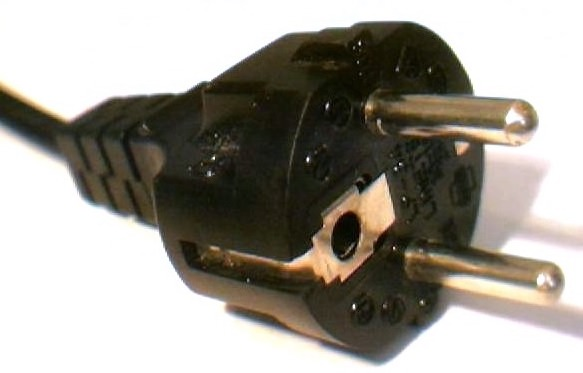
\includegraphics[scale=0.1]{type_e.jpg} \\
\bottomrule
\end{tabularx}
\end{table}

\subsection{Mise à la terre des appareils et structures conductrices}



\end{document}


%--------------------------------------
%conclusion, bibliographie
%--------------------------------------

\backmatter

	%--------------------------------------
	%inclusion des chapitres
	%--------------------------------------


	%--------------------------------------
	%bibliographie
	%--------------------------------------

	\nocite{AFPA2000, BourgeoisCogniel2005, CNED:SLT2003, Juguet2017, LyceeJean-Caillaud:PRE2013, Timin2003chap2, WildiSybille2014}
	
	\printbibliography %ajout des références bibliographiques
		
\end{document}

